% !TeX spellcheck = en_US
% !TeX encoding = UTF-8

\documentclass[
	paper=A4,
	twoside=true,
	openright,
	parskip=full,
	chapterprefix=true,
	11pt,
	headings=normal,
	bibliography=totoc,
	listof=totoc,
	titlepage=on,
%	draft
	final
	]{scrreprt}

\usepackage{lieb}
\graphicspath{{images/}}

\title{Development of a Fast Search Algorithm for the MUSiC Framework}
\date{09.09.2015}
\author{Jonas Lieb}

\makeatletter
\let\theauthor\@author
\let\thetitle\@title
\makeatother

\hypersetup{
	pdftex,
	pdfauthor={\theauthor},
	pdftitle={\thetitle},
	pdflang={en-US},
}

\begin{document}

\cleardoublepage
\pagenumbering{roman}
\pagestyle{empty}

\makeatletter
\begin{titlepage}
\begin{center}

\vspace{30mm}

\Huge \@title

\vspace{30mm}

\normalsize von \\

\vspace{5mm}

\LARGE \@author

\vspace{30mm}

\Large Bachelorarbeit im Fach Physik \\ \vspace{5mm}
\normalsize vorlegegt der \\
\Large Fakultät für Mathematik, Informatik und Naturwissenschaften \\
der RWTH Aachen \\ \vspace{5mm}
\normalsize im \\ \Large Juli 2015 \\ \vspace{5mm}
\normalsize angefertigt am \\ \Large III. Physikalischen Institut (IIIA) \\ \vspace{5mm}
\normalsize bei \\ \Large Prof. Dr. Thomas Hebbeker \vspace{5mm}

\end{center}
\end{titlepage}
\makeatother
\cleardoublepage
% !TeX spellcheck = de_DE
% !TeX encoding = UTF-8
% !TeX root = ../document.tex

Ich versichere, dass ich die Arbeit selbständig verfasst und keine anderen als die angegebenen Quellen und Hilfsmittel benutzt sowie Zitate kenntlich gemacht habe.

Aachen, den \todo{Datum}
\cleardoublepage

% !TeX spellcheck = en_US
\section*{Abstract}
The Model Unspecific Search in CMS (MUSiC) analyzes large amounts of LHC data by comparing kinematic distributions of the measured events to standard model predictions made by Monte Carlo simulations. Different from conventional dedicated analyses, MUSiC does not only focus on one or a few decay channels but covers a broad spectrum of final states which is considered. 
The calculation of the most significant deviations in the kinematic distributions is very computation intensive. This work features an additional selection step which significantly improves computation performance while keeping the same physical results: before the calculation of a complex integral, a simpler term is evaluated to estimate the significance of a certain region. The performance gain with this procedure is about \unit{XYZ}{\%} and will enable the MUSiC-group to perform more accurate analyses in the future.


% !TeX spellcheck = de_DE
\section*{Kurzdarstellung}


\cleardoublepage

\tableofcontents

\cleardoublepage
\pagenumbering{arabic}
\setcounter{page}{1}
\pagestyle{maincontentstyle}

% !TeX spellcheck = en_US
% !TeX encoding = UTF-8
% !TeX root = ../document.tex

\chapter{Introduction}

\section{Units}
Throughout this work, a natural unit system will be used, as it is convention in high energy particle physics. The speed of light and the reduced Planck constant are fixed to $c = 1$ and $\hbar = 1$, and as such they are omitted in equations. Additionally, energy is expressed in \GeV, where \unit{1}{\GeV} is the energy gain of an electron which is accelerated across a \unit{1}{\giga\volt} potential ($\unit{1}{\eV} \approx \unit{1.602 \e{-19}}{\joule}$). These conventions induce a change in units for the other dimensions, most importantly mass and momentum, both of which are notated in \GeV. Benefits of this choice of units are simpler equations, the possibility of a direct comparison between energy and masses, and typical quantities of $\order{\unit{1}{\GeV}}$.

\section{The Standard Model}
The \emph{standard model} (SM) is a theory that represents our current knowledge of elementary particles, their forces and interactions, excluding gravity. 

Particles in the standard model can be classified into two separate classes: \emph{Fermions}, which make up matter and possess a spin of \nicefrac{1}{2}, and \emph{bosons}, which are mediators of forces and possess an integer spin.
Three elementary forces arise, each from their separate theory: \emph{electrodynamic} (described by Quantum Electrodynamics, QED), \emph{strong} (described by Quantum Chromo Dynamics, QCD) and \emph{weak} (described by Quantum Flavor Dynamics). The forces are induced by corresponding charge-like properties: electrodynamic charge, color charge and weak isospin. These charges can then be used to further subdivide fermions into \emph{quarks} and \emph{leptons}, which will be described in the following sections. 

The standard model also provides theoretical predictions about the relations between particles, their masses and the probabilities of certain processes to happen. Because the probability is proportional to the number of times that a process occurs, experimentalists can validate the standard model by counting events with certain outcomes.

\subsection{Leptons}
There are three charged leptons: the \emph{electron} (\Pe), the \emph{muon} (\Pmu) and the \emph{tau} (\Ptau). They carry the electric charge of \unit{-1}{e} and participate in electrodynamic and weak interactions. For each charged lepton, there is one \emph{neutrino} counterpart (\Pnue, \Pnum, \Pnut). Neutrinos are electrically neutral, weakly interacting, massless particles. They remain undetected in current collider detectors.
The leptons do not carry color charge and are thus excluded from the strong interaction.
An overview about the leptons and their masses can be found in table~\ref{tbl:sm_leptons}.

\begin{table}[htb]
	\centering
	\begin{tabular}{ r | l | l | l | }
		\cline{2-4}
		& \multicolumn{3}{c|}{Leptons} \\ \cline{2-4}
		& electron (\Pe) & muon (\Pmu) & tau (\Ptau) \\ %\cline{2-4}
		mass & \unit{511.0}{\keV} & \unit{105.7}{\MeV} & \unit{1.777}{\GeV} \\ %\cline{2-4}
		charge & $-1$ & $-1$ & $-1$ \\ \cline{2-4}
		& \Pe neutrino (\Pnue) & \Pmu neutrino (\Pnum) & \Ptau neutrino (\Pnut) \\ %\cline{2-4}
		mass & $< \unit{2}{\eV}$ & $< \unit{0.19}{\MeV}$ & $< \unit{18.2}{\MeV}$ \\ %\cline{2-4}
		charge & 0 & 0 & 0 \\ \cline{2-4}
	\end{tabular}
	\caption{Leptons in the standard model\cite[p.~30, p.~690f.]{Oo2014Review}.}
	\label{tbl:sm_leptons}
\end{table}

\subsection{Quarks}
Similarly to the leptons, quarks can be divided into three generations. The first generation contains the stable \emph{up} and \emph{down} quarks, the second generation the \emph{charm} and \emph{strange} quarks and the third generation contains the heavy \emph{top} and \emph{bottom} quarks. Quarks carry a fractional electric charge of either \unit{\nicefrac{2}{3}}{e} or \unit{\nicefrac{-1}{3}}{e}.
They also carry color charges and take part in the strong interaction as well as in the weak interaction.
The three quark generations and their properties are shown in table~\ref{tbl:sm_quarks}.

\begin{table}[htb]
	\centering
	\begin{tabular}{ r | l | l | l | }
		\cline{2-4}
		& \multicolumn{3}{c|}{Quarks} \\ \cline{2-4} 
		& up (\Pup) & charm (\Pcharm) & top (\Ptop) \\ %\cline{2-4}
		mass & \unit{2.3}{\MeV} & \unit{1.28}{\GeV} & \unit{173.2}{\GeV} \\ %\cline{2-4}
		charge & \nicefrac{2}{3} & \nicefrac{2}{3} & \nicefrac{2}{3} \\ \cline{2-4}
		& down (\Pdown) & strange (\Pstrange) & bottom (\Pbottom) \\ %\cline{2-4}
		mass & \unit{4.8}{\MeV} & \unit{95}{\MeV} & \unit{4}{\GeV} \\ %\cline{2-4}
		charge & \nicefrac{-1}{3} & \nicefrac{-1}{3} & \nicefrac{-1}{3} \\ \cline{2-4}
	\end{tabular}
	\caption{Quarks in the standard model\cite[p.~33]{Oo2014Review}.}
	\label{tbl:sm_quarks}
\end{table}

\subsection{Bosons}
Gauge bosons are mediators of the elementary forces. The electromagnetic force is mediated by the massless \emph{photon} (\Pphoton), the strong force by the massless \emph{gluon} (\Pgluon) and the weak force by the massive \PZ and \PWpm bosons. They couple to the corresponding charges. To account for the massive boson masses, the Higgs mechanism is introduced. The Higgs field gives rise to the Higgs boson (\PHiggs), for which a candidate has been found in 2012\cite{Ao2015Combined}.
All bosons and their properties are listed in table \ref{tbl:sm_bosons}.

\begin{table}[htb]
	\centering
	\begin{tabular}{ r | l | l | l | l | l |}
		\cline{2-6}
		& \multicolumn{5}{c|}{Bosons} \\ \cline{2-6} 
		& Photon (\Pgamma) & Gluon (\Pgluon) & Z-Boson (\PZ) & W-Bosons (\PWpm) & Higgs (\PHiggs) \\ %\cline{2-6}
		mass & 0 & 0 & \unit{91.2}{\GeV} & \unit{80.4}{\GeV} & \unit{126}{\GeV} \\ %\cline{2-6}
		charge & 0 & 0 & 0 & $\pm 1$ & 0 \\ %\cline{2-6}
		force & el.-mag. & strong & weak & weak & Higgs \\ \cline{2-6}
	\end{tabular}
	\caption{Bosons in the standard model\cite[p.~27]{Oo2014Review}.}
	\label{tbl:sm_bosons}
\end{table}

\subsection{Antiparticles}
For each SM particle, there exists one counterpart with the same mass but an opposite sign for all charge-like properties, called \emph{antiparticle}. Unlike fermions, bosons are their own antiparticles, called Majorana particles.

\subsection{Ranges}
While the electrodynamic and weak couplings decrease with increasing distance, the strong force only grows stronger with a larger distance. This gives rise to the phenomenon of \emph{quark confinement}: as two quarks are separated from each other, new quark-antiquark pairs are created from the energy in between. Because of this, outgoing quarks with high energies form \emph{jets} consisting of hadrons from newly created quarks.

\section{The Large Hadron Collider}
Elementary particles and the standard model are commonly studied using scattering experiments. Such an experiment can be separated into two basic parts: an \emph{accelerator} and a \emph{detector}.
Inside the accelerator, the particles are accelerated to high energies using an electric field. They collide with their target inside the detector, which records various properties of the deflected or created particles, such as direction, momentum and energy. 
One can either accelerate particles on a straight line (\emph{linear accelerator}) or on a circular trajectory (\emph{ring}) which is enforced by dipole magnets. The latter option allows for longer acceleration time but is limited by the emission of Bremsstrahlung.
There are also two options for the collision. Either a \emph{fixed target} can be irradiated or two accelerated particle beams can be brought to collision (\emph{collider}). Because of kinematic reasons, a collider experiment can achieve higher energies.

\begin{figure}[htb]
	\centering
	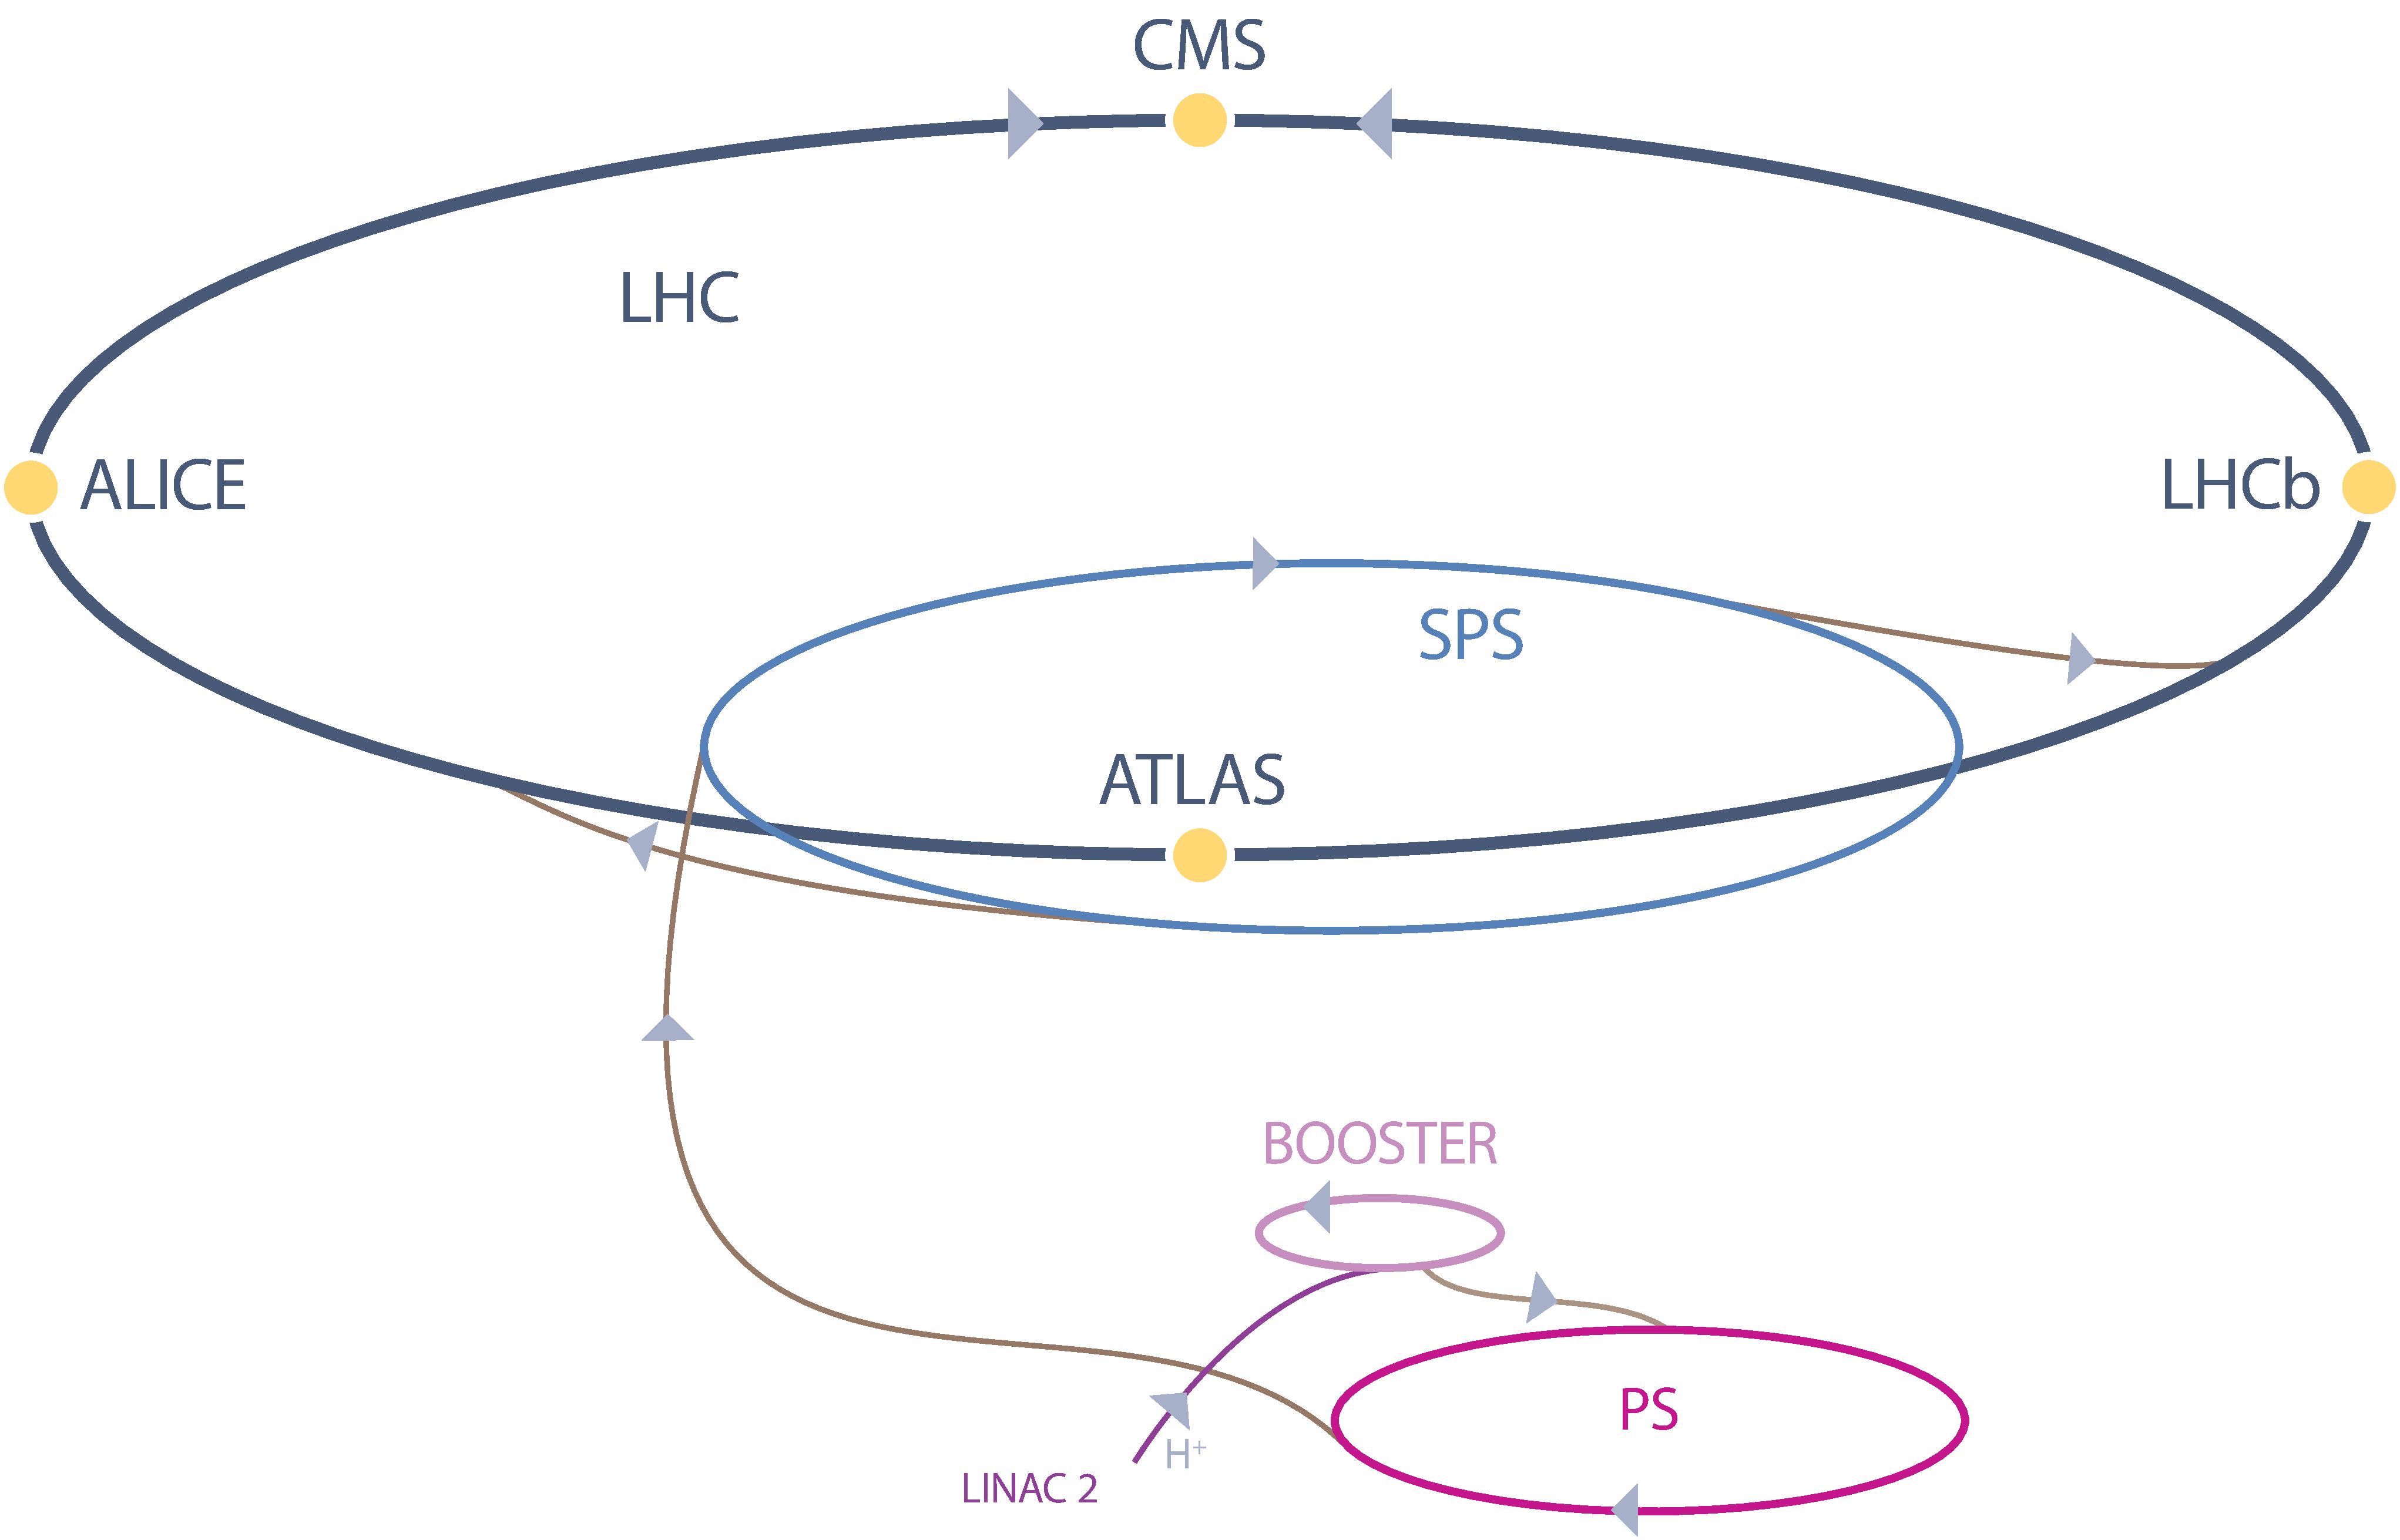
\includegraphics[width=0.5\linewidth]{CERN_accelerator_complex.pdf}
	\caption{The CERN accelerator complex\cite[modified]{Marcastel2013CERNs}. Shown are the LHC ring, the preaccelerators (Linear Accelerator 2, BOOSTER, Proton Synchrotron, Super Proton Synchrotron) and the four main LHC experiments: CMS, ATLAS, ALICE and LHCb.}
	\label{fig:cern_accelerator_complex}
\end{figure}

The \emph{Large Hadron Collider} (LHC) is a proton-proton ring collider experiment of the European Organization for Nuclear Research (\emph{Conseil Européen pour la Recherche Nucléaire}, CERN), situated between \unit{45}{\meter} and \unit{170}{\meter} underground near Geneva, Switzerland. The LHC has been installed in the tunnel of the former Large Electron Proton Collider (LEP), having a circumference of \unit{26.7}{\kilo\meter}\cite{BV2009CERN,EB2008LHC}. The two proton beams are injected into the LHC after passing a series of preaccelerators, as shown in figure \ref{fig:cern_accelerator_complex}. It has been designed to provide an energy of \unit{7}{\TeV} per beam, resulting in a center-of-mass energy $\sqrt{s} = \unit{14}{\TeV}$. It is currently (2015) running at $\sqrt{s} = \unit{13}{\TeV}$, the data analyzed in this work were taken in 2012 with $\sqrt{s} = \unit{8}{\TeV}$.

\section{The Compact Muon Solenoid Detector}
The Compact Muon Solenoid Detector (CMS) is an experiment at the LHC. The CMS detector\cite{Co2008CMS} consist of a barrel section along the beam pipe, which is closed off by two end caps. Collisions happen in the center of the barrel at the interaction point. 
The detector parts and particle footprints can be found in figure \ref{fig:cms_slice}.
Close to the \emph{interaction point}, the inner part of the barrel contains a \emph{silicon tracker} used to record trajectories of charged particles. 
The inner tracker is surrounded by an \emph{electromagnetic calorimeter} (ECAL) made of lead tungstate crystals. The ECAL measures energy deposited by electrons and photons, combined with the tracker it can distinguish between the two particle types. 
After the electromagnetic calorimeter follows the \emph{hadron calorimeter} (HCAL). It is a sampling calorimeter composed of layers of brass absorber plates and plastic scintillator fibers. Due to the high density of the brass absorbers, hadronic showers deposit most of their energy inside the HCAL.
The HCAL is surrounded by the most important feature of the CMS detector, the \emph{solenoid magnet}. The solenoid coil is cooled down below \unit{10}{\kelvin}, where the NbTi (Niobium-Titanium) conductor becomes superconducting, allowing for currents up to \unit{19}{\kilo\ampere}. The resulting field strength in the center of the coil is \unit{4}{\tesla}. The strong magnetic field causes the charged particle tracks to bend, this effect is used to measure the momentum of charged particles.
In the outer part one finds the iron return yoke interspersed with \emph{muon drift chambers}, \emph{cathode strip chambers} and \emph{resistive plate chambers}. Since only muons and neutrinos pass through the solenoid and iron yoke and neutrinos remain undetected, the drift chambers can precisely identify muons and assess their momentum.

\begin{figure}[htb]
	\centering
	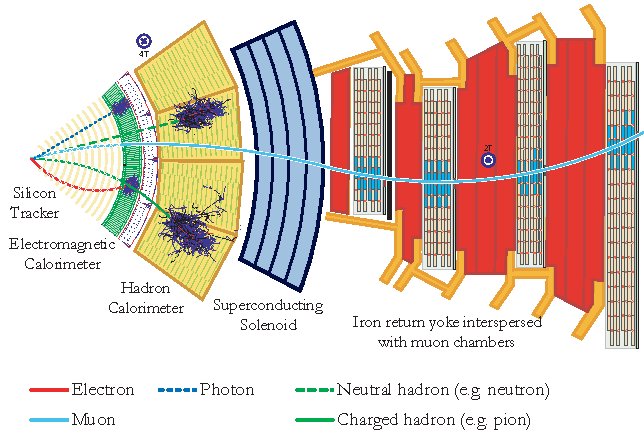
\includegraphics{CMS_Slice.pdf}
	\caption{Slice through the CMS detector. The different detector layers (tracker, ECAL, HCAL, magnet, muon chambers) are shown, alongside schematic tracks of an electron, a photon, a charged and neutral hadron and a muon.\cite[modified]{Barney2011CMS}}
	\label{fig:cms_slice}
\end{figure}

\subsection{Coordinate System}
The CMS collaboration has defined a spherical coordinate system inside the detector, as illustrated in figure \ref{fig:cms_coordinate_system}. The origin is located in the interaction point, the z-axis points along the beam pipe towards the Jura mountains. The x-axis is defined towards the center of the LHC ring. To complete the right-handed orthogonal coordinate system, the y-axis points upwards, orthogonally from the x-z-plane. 
An azimuthal angle $\phi$ is defined from the x-axis in the x-y plane. The polar angle $\theta$ is measured from the z-axis. One can also define a radial coordinate $r$ in the x-y plane, as distance from the z-axis.\cite[p. 2]{Co2008CMS} 
\begin{figure}[htb]
	\centering
	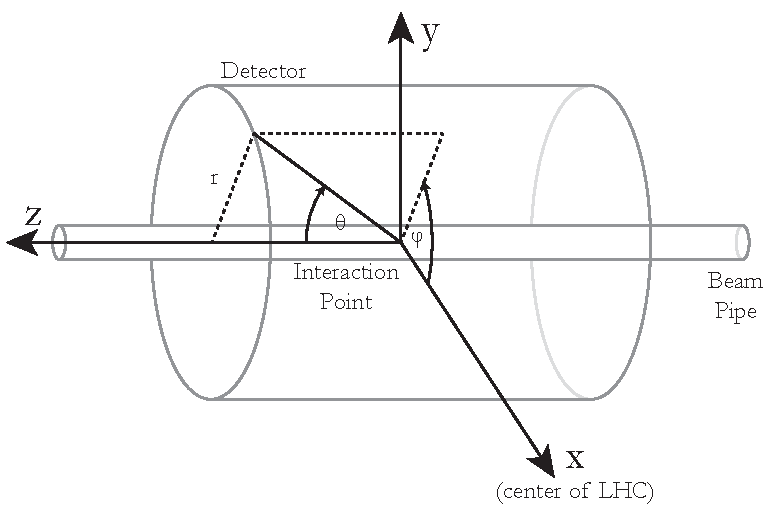
\includegraphics[width=0.9\linewidth]{CMS_coordinate_system.pdf}
	\caption{The CMS coordinate system.}
	\label{fig:cms_coordinate_system}
\end{figure}

\section{Commonly Used Quantities}
The proton is a composite particle consisting of quarks and gluons, which each carry an unknown momentum fraction. Because a collision can only occur between these constituents, the initial momentum sum along the z-axis is unknown.
Thus, most of the kinetic variables are defined in the transverse (x-y) plane. A particle is assigned a \emph{transverse momentum} \pT which only contains the transverse component of its momentum vector. Analogous, only a fraction of the energy is regarded, the \emph{transverse energy} \ET. 
The sum of all transverse momenta in a final state is usually not equals to zero since invisible neutrinos carry away some of the momentum. This is accounted for by the negative sum of the transverse energy, which is called \emph{missing transverse energy} \MET.
Another commonly used quantity is the pseudo-rapidity $\eta = -\ln \tan(\theta/2)$, which has the property that distances $\Delta\eta$ are Lorentz invariant.

\section{Bunch Crossings, Events, Collisions and Pileup}
For acceleration purposes, the protons circulating in the LHC beam pipe are grouped into 2808 \emph{bunches}\cite[p.4]{EB2008LHC}. A \emph{bunch crossing} happens every \unit{50}{\nano\second} (2012), defining an \emph{event}. During an event, multiple pp-collisions can occur. The collision containing the vertex with the highest energy is called \emph{hard interaction}. All other collisions that do not correspond to the physics process of the hard interaction are classified as \emph{pileup}.

\section{Trigger}
Since the raw data for each event is about $\order{\unit{1}{\mega\byte}}$, the throughput required to transfer all data would be $\order{\unit{20}{\tera\byte}}$ per second. This amount of data is too much for current hard- and software, thus a selection mechanism is introduced to match the amount of recorded data to the networking, processing and storage capabilities. This system is called \emph{trigger}. The CMS trigger system consists of two layers, the "Level-1 Trigger" (L1), implemented in hardware on site, and the software "High-Level-Trigger" (HLT), located at a computing farm close to the detector. The triggers process the limited input from the detector and decide whether an event is worth storing on disk, based on physics arguments. These requirements reduce the data amount by $\order{10^{-6}}$.

\section{Event Reconstruction}
Various \emph{reconstruction} (RECO) algorithms are executed offline to reconstruct physics objects from the recorded data. The most important inputs are the bending radius of the particle tracks, energy deposits in the calorimeters and hits in the muon chambers. 
A notable algorithm that ensures that each input is linked to exactly one physics object has been developed by CMS and is called \emph{Particle-Flow}\cite{2009Particle}. 
% !TeX spellcheck = en_US
% !TeX encoding = UTF-8
% !TeX root = ../document.tex

\chapter{Model Unspecific Search in CMS}

The Model Unspecific Search in CMS (\emph{MUSiC}) is an analysis procedure that compares observed data to Monte Carlo (MC) expectations of the standard model. Unlike dedicated analyses that usually only regard a few decay channels, an unspecific search covers a broad spectrum of final states. Because MUSiC is sensitive to small deviations that occur in multiple decay channels, it is well suited for searches for processes that are not significant at low-energy scales.

This chapter will focus on the existing MUSiC workflow. First, the motivation behind an unspecific search will be illustrated, then the three steps \emph{skimming}, \emph{classification} and \emph{scanning} will be explained\cite{Pieta2012MUSiC,Papacz2014Model}.

\section{Motivation}
Since a Higgs boson candidate has been discovered at the LHC\cite{Ao2015Combined}, all predicted SM particles have been observed. Particularly in this time, questions about new physics beyond the standard model (BSM) arise. 
BSM phenomena include unification theories, heavy "copies" of the vector bosons (\PZprime, \PWprime), supersymmetric extensions to the SM (SUSY), string theories and quantum black holes.
Expected signatures of these models would show up in a large range of final states. For some models, narrow resonances are predicted, other result in a slight signature in the high-energy tail of the distributions.
The MUSiC analysis is sensitive to these kind of deviations.
Additionally, MUSiC can identify deviations between MC and data that originate from non-physics sources, uncovering weaknesses in the Monte Carlo simulation.

\section{Skimming}
The goal of skimming is to gather events from different data sources and convert them to a unified format containing only information relevant to MUSiC. AOD (analysis object data) files of observed as well as simulated events are downloaded from the computing grid to the local cache, where unnecessary information is stripped from the events. If the skimmed dataset originates from MC simulations, it is rescaled and shifted within its systematic uncertainties.
The resulting files are stored in the PXL I/O format\cite{BBE+2012Development}.

\section{Classification}
During the classification step, events are grouped into \emph{event classes} (EC) according to their physics content in the final state. 
Missing transverse energy is treated as separate physics object. There are three  types of event classes: \emph{exclusive}, \emph{inclusive} and \emph{jet inclusive}. Final states of events in exclusive event classes contain exactly the objects indicated in the event class name. 
Events in the exclusive EC \eventclass{1e + 1MET} contain only 1 electron and missing transverse energy in the final state, but no other physics objects.
Events in the inclusive EC can contain any other objects besides the indicated ones. \eventclass{1e + 1MET + X} contains at least 1 electron and missing transverse energy. 
Additionally, there are \emph{jet inclusive} event classes (e.g. \eventclass{1e + 1MET + Njet}), that exclusively contain the mentioned objects and zero or more jets, making the analysis more robust to initial and final state radiation caused by the emission of a gluon in the initial or final state.

These definitions imply that each event is contained in exactly one inclusive EC, at least one exclusive EC and at least one jet inclusive EC.

The classification algorithm automatically adjusts the possible event classes to the events actually contained in the dataset, spontaneously creating new classes. It also makes sure that events are only considered once, even if they have been stored by two separate triggers.

\subsection{Kinematic distributions}
For each event class, a histogram of the kinematic variables \sumpT, \Minv, \MET is calculated. The histograms are created with variable bin sizes according to the detector resolution\cite[p. 52]{Papacz2014Model}. Note that the vertical axis of histograms shown in this work carries the unit "Counts per \unit{10}{\GeV}", so to get the absolute number of events in a bin, the vertical data point has to be multiplied by the width of its bin.

% MUSiC/EventClassFactory/Resolutions.hh als Quelle
% Pauls Dis durchlesen
% AN: file:///T:/Temp/Downloads/AN2014_098_v5.pdf

\section{Scanning}
The scanning algorithm (\emph{scanner}) searches for the most significant deviation between MC and data in each histogram.

\subsection{Region Building}
For each histogram, the scanner probes all connected bin regions and calculates the \p~value for each one.

The set of connected bin regions can be defined and calculated as
\begin{equation}
R = \{(s, e) \, \forall e \in (s + m, l) \, \forall s \in (0, l-m)\}
\end{equation}
where the histogram spans the bins $0$ to $l$ and $m$ denotes a minimal number of bins per region which can be configured.

For each region, the \p~value is calculated. The region of most deviation (smallest \p) is called \emph{region of interest} and stored.

\subsection{The \p value}
Given the number of total events in a region~\Ndata and an expectation~$\Nmc \pm \sigmamc$, the \p value expresses the probability of making this measurement or a more significant one.
Since the calculation deals with results of counting experiments, a Poisson distribution is assumed. The probability of making an observation $N$ given the Poisson mean~\Nmc is
\begin{equation}
	P(N) = \frac{e^{-\Nmc} \Nmc^N}{N!}
\end{equation}
To include observations that are more extreme than the observation, the probabilities are summed away from the expectation:
\begin{equation}
p = 
	\begin{cases} 
		\displaystyle
		\sum\limits_{N = \Ndata}^{\infty} \frac{e^{-\Nmc} \Nmc^N}{N!} &\mbox{if} \; \Ndata \geq \Nmc \\
		\displaystyle
		\sum\limits_{N = 0}^{\Ndata} \frac{e^{-\Nmc} \Nmc^N}{N!} &\mbox{if} \; \Ndata < \Nmc
	\end{cases}
\end{equation}
Since the Poisson mean is usually not exactly known, for example because of Monte Carlo statistics, it is evaluated for multiple possible values $\theta$ which are weighted by a Gaussian distribution of width~\sigmamc around \Nmc. This final probability is called \emph{\p value}:
\begin{equation}
p \defeq 
	\begin{cases} 
		\displaystyle
		\sum\limits_{N = \Ndata}^{\infty} C \cdot \int\limits_0^\infty \dd \theta \exp(-\frac{(\theta-\Nmc)^2}{2 \sigmamc^2}) \cdot \frac{e^{-\theta} \theta^N}{N!} &\mbox{if} \; \Ndata \geq \Nmc \\
		\displaystyle
		\sum\limits_{N = 0}^{\Ndata} C \cdot \int\limits_0^\infty \dd \theta \exp(-\frac{(\theta-\Nmc)^2}{2 \sigmamc^2}) \cdot \frac{e^{-\theta} \theta^N}{N!} &\mbox{if} \; \Ndata < \Nmc
	\end{cases}
\end{equation}
The constant $C$ denotes a normalization factor that compensates for using $0$ as the lower limit of the integral. This is necessary since the Poisson distribution with a negative expectation is not physical.

\subsection{The \ptilde value}
For a dedicated analysis looking at one fixed histogram region only, this \p~value would be sufficient to describe the statistical significance of the deviation. But since the scanner algorithm regards many regions to choose the most significant one from, the probability of finding a deviation somewhere is larger than \p. This is called \emph{look elsewhere effect}.

To counter the look elsewhere effect, the scanning algorithm is applied multiple times on randomly diced pseudo-data. For each pseudo experiment, first the expected mean $\Nmc'$ is randomly shifted from a Gaussian distribution around \Nmc, having the width of the systematic error \sigmamc. Taking this new pseudo-mean, a random Poisson number is chosen as new observed value $\Ndata'$. The dicing of pseudo experiments is performed in a correlated way, the choice of $\Nmc'$ is shared between all distribution in all event classes. The complete scanning algorithm is repeated for each pseudo-experiment, finding a region of interest and its \p value.
\begin{figure}[htbp]
	\centering
	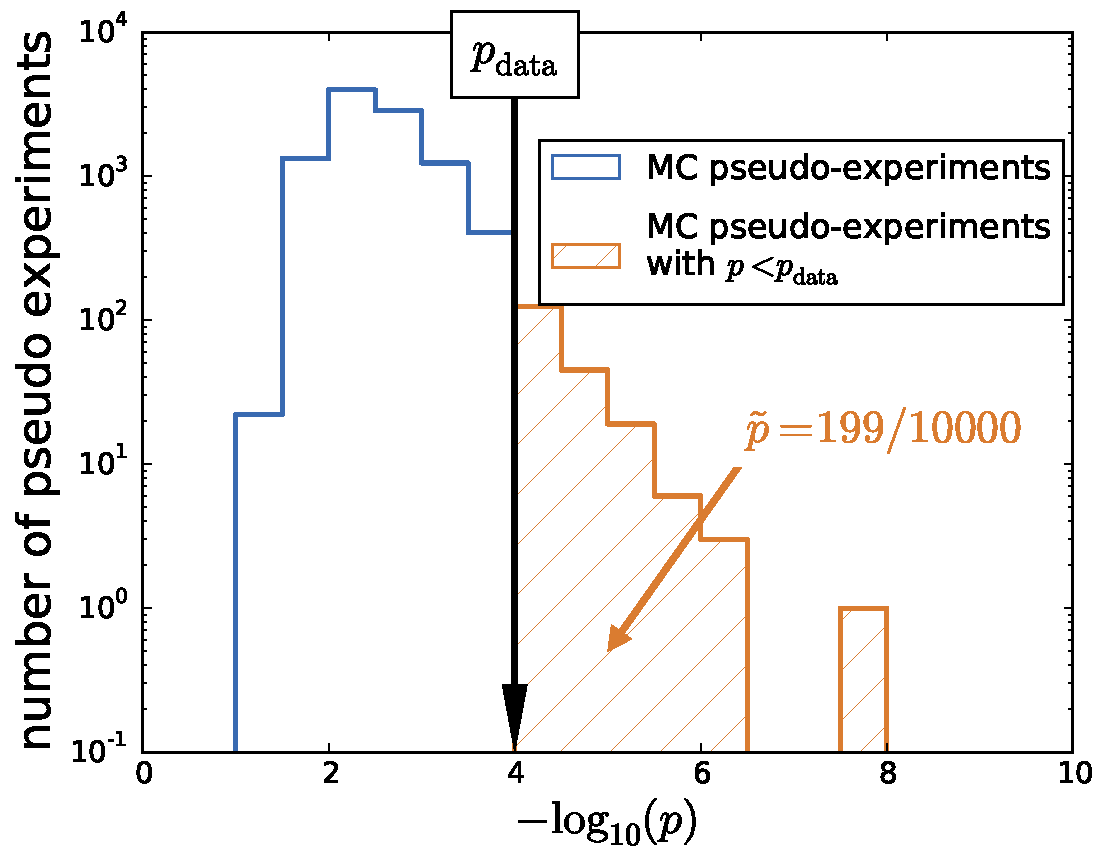
\includegraphics[width=0.6\textwidth]{ptilde_illustration.pdf}
	\caption{Illustration of a \ptilde calculation. 1000 pseudo-experiments have been conducted. The XYZ experiments on the right of $p_\mathrm{data}$ have shown a more extreme deviation somewhere in the distribution.\todo{generate graphics to insert here}}
	\label{fig:ptilde_illustration}
\end{figure}
Finally, the amount of pseudo experiments with more significant deviations is compared to the total amount of pseudo experiments conducted:
\begin{equation}
	\ptilde \defeq \frac{\text{number of pseudo-experiments with } \p < \p_\mathrm{data}}{\text{total number of pseudo experiments}}
\end{equation}
This \ptilde~value is used as significance indicator throughout other MUSiC publications.





% !TeX spellcheck = en_US
% !TeX encoding = UTF-8
% !TeX root = ../document.tex

\chapter{Motivation for a Fast Search Algorithm}
\label{ch:quickkscan_motivation}

The calculation of the \p~value includes integration over a series. The \p~value is calculated for each connected bin region, resulting in a runtime of $\order{n^2}$ with the number of bins in a distribution. Additionally, the runtime increases linearly with the number of classes, distributions and pseudo-experiments.

The typical number of integrals computed during a full scan of 2012 data, one kinematic variable and $10^5$ pseudo-experiments is $\order{10^{9} - 10^{10}}$. Table \ref{tbl:motivation_timing} shows that the computation of each single integral takes about \unit{200}{\micro\second}, which results in a total computation time of about 2 to 20 CPU-days. The scan is usually performed on a 64 core machine and thus takes between 1 and 9 hours wall-time.

The calculation of the integral is performed using simple adaptive integration (QAG, from the GNU Scientific Library). Since this implementation is already highly optimized, further improvement is difficult.

The fast search algorithm, called \emph{Quickscan} in this work, aims to reduce the number of integrals by cutting down the number of region of interest candidates for which the \p~value is calculated. It shall not reduce the amount of regions so far that the "true" region of interest is not included anymore, since this would highly impact physics accuracy and will be closely examined in the remainder of this work.

Shortening the scanning time will eventually enable the MUSiC project to increase the number of pseudo experiments and remove other requirements that have been made for optimization, but have a higher impact on physics accuracy.

\begin{table}[htbp]
	\centering
	\begin{tabular}{| r | r || r |}
		\hline
		Number of integrals & Total runtime & Time per integral \\
		\hline \hline
		23110209 & \unit{5179.87}{\second} & \unit{224}{\micro\second} \\
		81734778 & \unit{16983.60}{\second} & \unit{207}{\micro\second} \\
		\hline
	\end{tabular}
	\caption{Benchmarking results of the original scanning process. The timing has been measured on a data subset, as wall-time, using a single CPU and includes setting up the process and writing out the results. The agreement of the time per integral between the runs motivates the rough estimate of \unit{200}{\micro\second} per integral.}
	\label{tbl:motivation_timing}
\end{table}
% !TeX spellcheck = en_US
% !TeX encoding = UTF-8
% !TeX root = ../document.tex

\chapter{A Fast Search Algorithm}

In this chapter, the basic concept and method of the Quickscan algorithm is described. Arising problems and their solutions within the algorithm are proposed. Finally, other approaches are mentioned, which have not been implemented in this works version of Quickscan.

\section{Concept}
The goal of the Quickscan algorithm is to make the scanning process of pseudo-experiments more efficient. The efficiency improvement is achieved by preselecting interesting regions as RoI (region of interest) candidates and discard most other regions before the costly \p~value calculation.
The selection is performed by evaluating a less computation intensive estimator over all possible connected regions, and making a selection of the most significant deviations according to this estimator. Finally, the full \p~value and its integral are only calculated for the few candidate regions returned by the estimator.

\subsection{The Estimator}
The choice of the estimator plays an important role in the efficiency of the selection. A commonly used quantity in particle physics is 
\begin{equation}
\mychi = \frac{|\Ndata - \Nmc|}{\sigmamc'}
\end{equation}
Here the value $\sigmamc'$ describes the expected deviation. This is not $\sigmamc$, because that value only includes systematic uncertainties, e.g. finite Monte-Carlo statistics, and has been scaled by the luminosity.
$\sigmamc'$ consists of the expected statistical deviation $\sqrt{\Nmc}$ and the systematical error $\sigmamc$. The two errors are added quadratically. Because $\Nmc \geq \num{0}$, the expression can be simplified:
\begin{equation}
\sigmamc' \defeq \sqrt{\sigmamc^2 + \left(\sqrt{\Nmc}\right)^2} = \sqrt{\sigmamc^2 + \Nmc}
\end{equation}

This value incorporated into the \mychi-value gives
\begin{equation}
\mychi = \frac{|\Ndata - \Nmc|}{\sqrt{\sigmamc^2 + \Nmc}}
\end{equation}

\subsection{Selection}
In each distribution, the \mychi~value is calculated for each connected bin region. The most significant regions are stored in a list. This introduces a parameter of the Quickscan algorithm, \paramregions, which denotes the \emph{number of candidates} kept in the list.

\subsection{Nested Region Handling}
Using only the estimator and the selection of top \paramregions candidates, the algorithm tends to get stuck around single data points in the tail of the distribution. This is illustrated in figure \ref{fig:no_nested_region_handling}. 
\begin{figure}[htb]
	\centering
	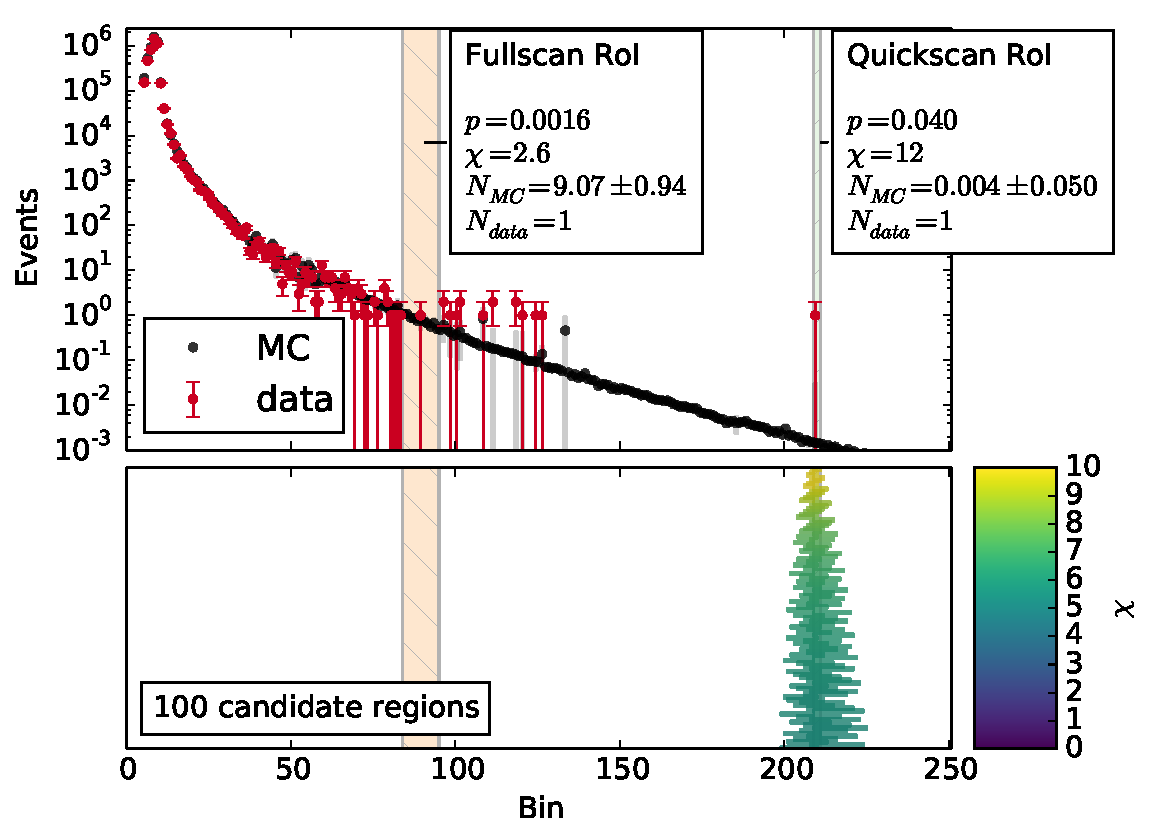
\includegraphics{no_nested_region_handling}
	\caption{Example distribution: pseudo experiment of the \eventclass{2e} \sumpT distribution, without special treatment of nested regions. The upper panel shows the distribution with the bin number (not the physical quantity) on the horizontal axis and the number of events in each bin on the vertical axis. The lower panel shows the \num{100} selected candidate regions, sorted by \mychi. The regions chosen by the different approaches are indicated in the upper panel. One can see that especially in the regions with \numrange{0}{3} expected events, where the Poissonian approach $\sigma_N = \sqrt{N}$ fails, the \mychi value is too sensitive. The nested regions suppress different regions in the candidate list, such that the "true" RoI (as found without the Quickscan) is not detected.}
	\label{fig:no_nested_region_handling}
\end{figure}
The pseudo experiment of the \eventclass{2e} \sumpT distribution shows a single event above a low background expectation. The regions with the highest \mychi gather around this excess. Comparison with a scan without the new algorithm shows that the "true" region of interest is found further left in the distribution, as a deficit with only \num{1} observed event in \num{9} expected.

To suppress this behavior, an additional list of criteria is introduced, comparing region $A$ with region $B$:
\begin{my_list}
	\item $A$ is nested inside of $B$
	\item excess of data in $A$: $\Ndata(A) > \Nmc(A)$
	\item excess of data in $B$: $\Ndata(B) > \Nmc(B)$
	\item no additional data in $B \setminus A$: $\Ndata(A) = \Ndata(B)$
\end{my_list}
If all these conditions are met, then region $A$ is more significant than region $B$.
The mathematical proof for this criterion is difficult, but it can be motivated as follows: if a region contains an excess of observed event yield over MC event yield, and the region is extended while the amount of observed events remains the same, the difference between \Nmc and \Ndata stays equal or is reduced. Since the error \sigmamc can only stay the same or increase, the total significance of the extended region must be less than the original region, as long as it still contains an excess.

\begin{figure}[htb]
	\centering
	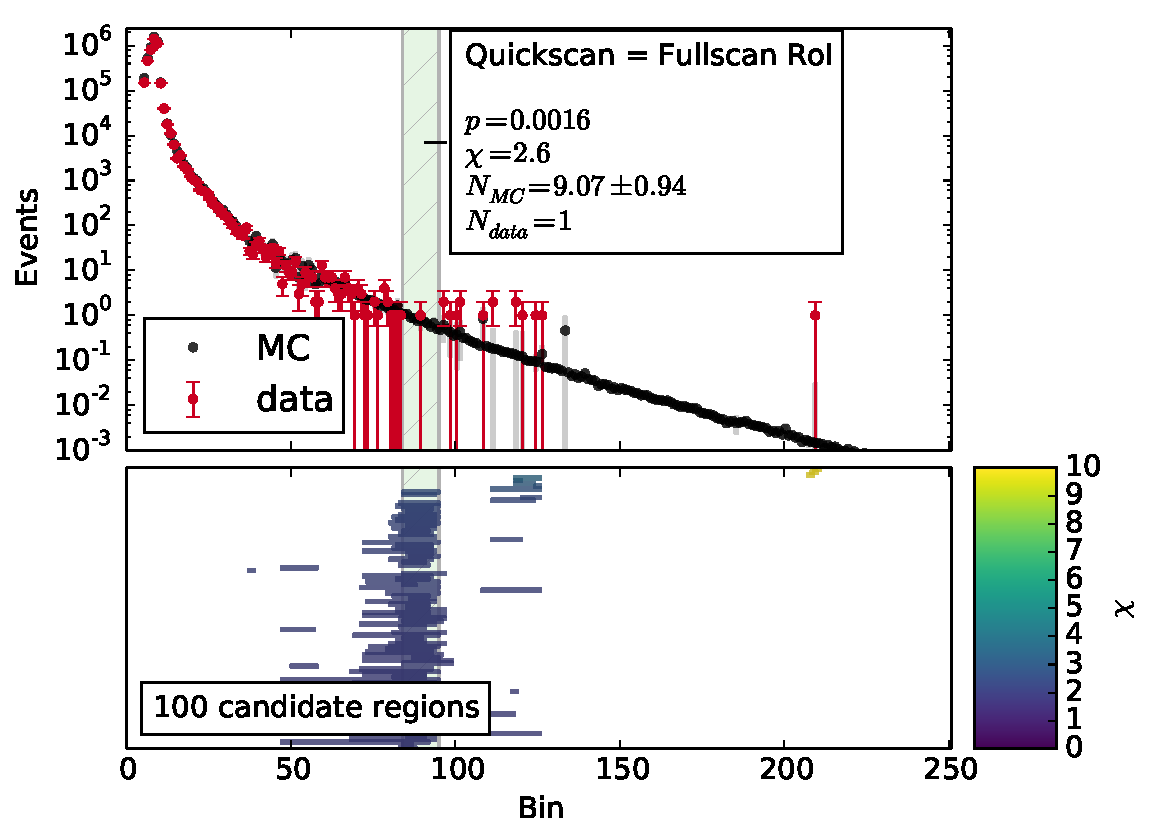
\includegraphics{with_nested_region_handling}
	\caption{Example distribution: pseudo experiment of the \eventclass{2e} \sumpT distribution, with special treatment of nested regions. The scheme is explained below figure \ref{fig:no_nested_region_handling}. }
	\label{fig:with_nested_region_handling}
\end{figure}
Based on this comparison, regions are immediately rejected if a more significant subregion is already included in the candidate list. The results of this treatment can be observed in figure \ref{fig:with_nested_region_handling}. The distribution is exactly the same as in \ref{fig:no_nested_region_handling}, but the algorithm does not focus overly on the event in the tail, leading to the correct RoI to be found.

%\subsection{Magnitude Binning}
%Ideally, the estimator should indicate significance in the same way as the \p~value. For this to work, there should be a monotonous functional dependency $\p(\mychi)$. To investigate this, one can plot \mychi vs. \p (figure \ref{fig:pvschi_vary_data}). In this illustration, \Nmc and \sigmamc are set to fixed values and \Ndata is varied. 
%\begin{figure}[htb]
%	\centering
%	\includegraphics{pvschi_vary_data}
%	\caption{Dependency of the \mychi~value and the \p~value. No physics data is involved, instead the value \Nmc and \sigmamc have been fixed and the amount of data \Ndata was varied in integer steps. With an optimal estimator, there should be no dependency on \Nmc, and all lines should align on top each other, with \mychi monotonically decreasing with \p.}
%	\label{fig:pvschi_vary_data}
%\end{figure}
%
%The first conclusion that can be drawn from this plot is that there is no trivial dependency $\p(\mychi)$. The significance expression depends on \Nmc, such that the best dependency can be $\p(\mychi, \Nmc, \sigmamc)$.
%A second conclusion is that for a fixed value of \Nmc, the dependency is monotonous. Thus, when comparing regions with the same value of \Nmc, \mychi is a valid indicator for significance which could be directly related to \p.
% 
%These conclusions motivate a solution called \emph{magnitude binning}.
%In order to only compare regions with approximately the same \Nmc, Quickscan first determines the magnitude $\log(\Nmc)$. For each magnitude, a separate list of \paramregions regions is maintained. 
%The index $i$ of each bin is calculated as 
%\begin{equation}
%i = \floor{\log_\parambinbase(\Nmc)} = \floor{\frac{\log(\Nmc)}{\log(\parambinbase)}}
%\end{equation}
%Here, a new parameter of the Quickscan algorithm, \parambinbase, has been introduced. It controls the size of the magnitude bins.
%
%\subsection{Separation of Excesses and Deficits}
%Figure \ref{fig:pvschi_vary_data} also shows that for a constant magnitude of \Nmc, $\p(\chi)$ has two branches which correspond to excesses and deficits. Because of this, each magnitude bin is again split into two separate candidate lists containing \paramregions regions each.

\section{The Final Algorithm}
The solutions suggested in this chapter are combined in the final algorithm: the Quickscan algorithm maintains a single list of \paramregions candidates for each distribution in each class. Every time a new candidate is considered for insertion into the list, first the nested region criteria are evaluated. If the region is not nested inside any other region in the list, its \mychi~value is computed and compared to the candidates in the list. If it is larger than the lowest \mychi inside the list, the region is swapped into the list.

After all connected regions have been considered, the \p~value is evaluated for the candidate collection and the final region of interest is determined as one of the candidates. 

\section{Preserving the \p~Value of Data}
The Quickscan method is only applied to pseudo-experiments, not when calculating the \p~value of measured data, since there might still be cases in which a scan using Quickscan does not find the same region of interest as without. This assures that the data region of interest and its \p~value are definitely correctly computed.

\section{Other Investigated Approaches}
Another method that has been considered during this work is \emph{Magnitude Binning}. This ad-hoc solution also targets the low-statistic regions by differently treating regions with different \Nmc. Instead of keeping one candidate list for an entire distribution, Magnitude Binning keeps one candidate list for each magnitude of \Nmc. The magnitude index is calculated as
\begin{equation}
i = \floor{\log_\parambinbase(\Nmc)} = \floor{\frac{\log(\Nmc)}{\log(\parambinbase)}}
\end{equation}
This introduces a new parameter, \parambinbase, which indicates the size of a magnitude bin. Additionally, the total number of candidate regions is increased by an unknown amount, since the number of orders of magnitude are originally unknown.

This method has been dropped since the methods proposed in this chapter sufficiently satisfy the Quickscan goals. The Magnitude Binning extension only introduces unnecessary complexity and an additional parameter.


% !TeX spellcheck = en_US
% !TeX encoding = UTF-8
% !TeX root = ../document.tex

\chapter{Optimization of the Algorithm}
In this chapter the optimal value for the Quickscan parameter \paramregions is determined. This value highly impacts performance and physics accuracy. Possible approaches for a trade-off between speed and quality will be proposed.

\section{Metrics}
The optimization is performed in regard of the goals described in chapter \ref{ch:quickkscan_motivation}: physical performance and required computation time.

\subsection{Physics Sensitivity}
The physics sensitivity is measured as deviation of \ptilde. To calculate this deviation, the sample scanning run is compared to a reference run with the same settings but without the Quickscan procedure. Since the \ptilde~value is only evaluated for distributions with a RoI \p~value of $< 0.3$, the reference as well as the sample run only contain \ptilde~values for a subset of event classes (usually about half).

For each event class, the \ptilde~value of the reference run is compared to the corresponding \ptilde~value of the trial run:
\begin{equation}
	\sigma_\mathrm{rel} = \frac{\Delta \ptilde}{\ptilde_\mathrm{reference}} = \frac{\ptilde_\mathrm{sample} - \ptilde_\mathrm{reference}}{\ptilde_\mathrm{reference}}
\end{equation}

\begin{figure}[htbp]
	\centering
	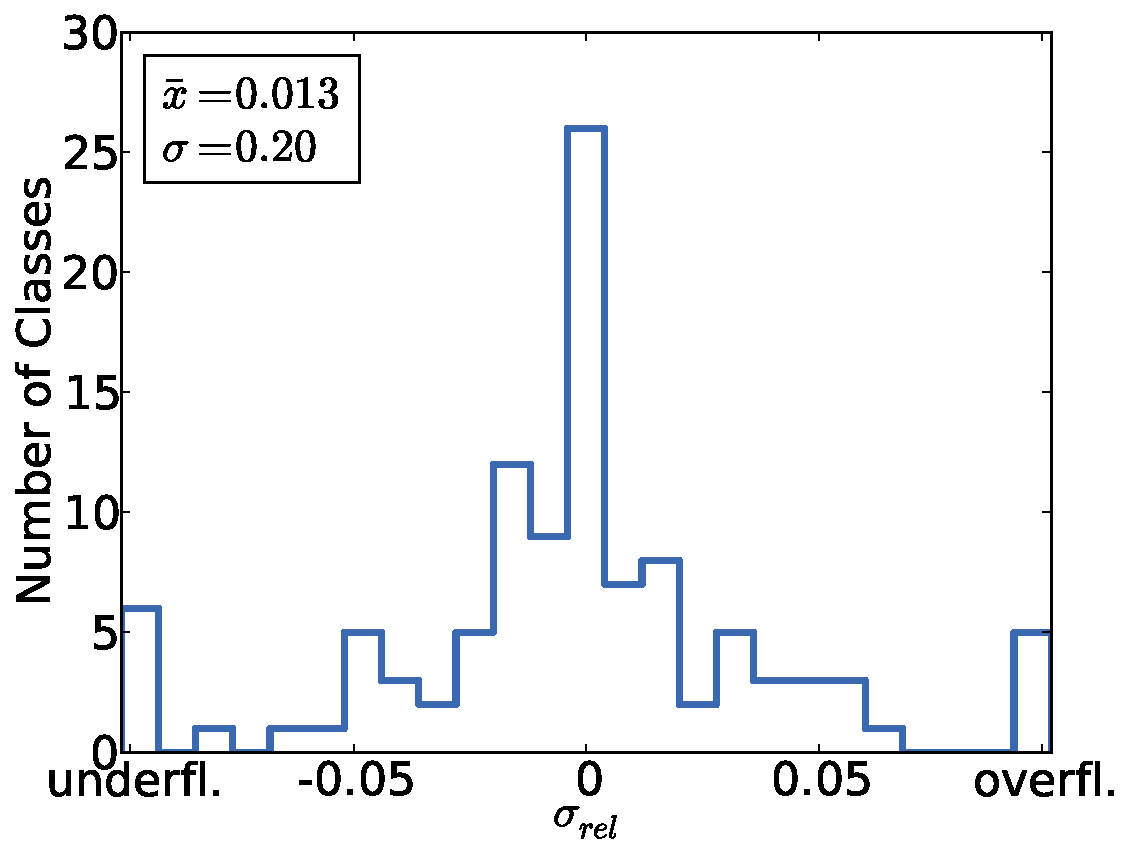
\includegraphics{delta_p_tilde_random_deviation}
	\caption{Random deviation of $\sigma_\mathrm{rel}$. Obtained by comparing two sets of scan results without the Quickscan algorithm. The distribution spread of $\order{\unit{5}{\%}}$ originates in the random means of the pseudo experiments. This also demonstrates that only 16 classes show no deviation at all.}
	\label{fig:delta_p_tilde_random_deviation}
\end{figure}

Figure \ref{fig:delta_p_tilde_random_deviation} shows the deviation of $\sigma_\mathrm{rel}$ caused by random dicing of pseudo experiments while calculating \ptilde (see section \ref{sec:music_ptilde}). The conclusion of this illustration is that dicing the pseudo-experiments introduces a statistical uncertainty of $\order{\unit{5}{\%}}$ on the \ptilde~value. This value will act as guideline for the Quickscan parameter choice.

\subsection{Computation Time}
There are various approaches to the comparison of computation costs of computer programs: A commonly used option is to count the number of CPU cycles that a program has used. This method allows for comparisons with a high resolution, but this "pure" CPU time does not represent the time spent on a real-world application. Additionally, it is more difficult to implement, especially in an environment like the MUSiC scanning algorithm because of multitasking and the usage of various technologies (Python and C++). 

The alternative technique used in this work is \emph{wall-clock time}. The measurement of wall-clock time is performed by acquiring a timestamp before and after the execution of the program. The elapsed time is the difference between those two timestamps. The results of such measurement can be directly transfered to the real-world application because it is performed in the same environment as an execution on a user machine.

This method introduces the following systematic uncertainties:
\begin{my_list}
	\item CPU usage by other processes: The measurement is performed on a system shared by multiple users. The operating system distributes the available CPU resources between the user processes. Thus, the benchmarked program runs significantly slower if other computation intensive processes are present. In order to suppress this effect, it is ensured that at the time of the measurement, the machine is not occupied by other users. The influence can be lowered this way, from $\order{10^{-1}}$ to $\order{10^{-2}}$.
	\item IO throughput: The files required by the scanning algorithm are stored on shared network drives. Similarly to the CPU usage, the behavior of other users influences the measured wall-time (also $\order{10^{-2}}$).
	\item Static overhead: The measurement includes operations that are not being optimized and contribute a constant amount of time. Examples are reading and parsing of parameters and configuration, creating and destroying multitasking worker processes and writing output files. This takes up $\order{10^{-2}}$ of the total time but is expected to be almost constant.
	\item Timestamp resolution: Although the operating system's internal clock has a high resolution, the results are only written to file with a resolution of \unit{1}{\second}. In comparison to the other uncertainties, this is negligible ($\order{10^{-4}}$). 
	\item Time adjustments: The time on the computing host is managed by the Network Time Protocol (NTP). It ensures time synchronization inside the datacenter. If the NTP daemon notices that either the time of the host has shifted or if leap seconds are introduced, the host time is adjusted. This has an effect on the acquired timestamps but is highly negligible in this scenario ($\order{10^{-6}}$).
\end{my_list}

The computation improvement is quantified by the ratio between the wall-clock time measurement of the full scan and the Quickscan algorithm:
\begin{equation}
	\textrm{speedup} = \frac{T_{\textrm{classic}}}{T_{\textrm{quickscan}}} \geq 1 
\end{equation}


\section{Optimization Environment}
The optimization is performed in 60 processes on a 64-core MUSiC host, whose specifications are listed in table \ref{tbl:music_machine}. The wall-time is measured for the entire execution of the main scanning script, \texttt{MISMaster.py}.

\begin{table}
	\centering
	\begin{tabular}{r|l|}
		\cline{2-2}
		host & lx3acms1.physik.rwth-aachen.de \\
		\cline{2-2}
		processors & AMD Opteron Processor 6272 \\
		clock speed & \unit{2.1}{\giga\hertz} \\
		cores per CPU & 8 logical (4 physical) \\
		total number of cores & 64 \\
		memory & $\approx \unit{250}{\giga\byte}$ \\
		\cline{2-2}
		operating system & Linux \\
		kernel version & 2.6.32-504.16.2.el6.x86\_64 \\
		distribution & Scientific Linux release 6.5 (Carbon) \\
		\cline{2-2}
		CMSSW version & 5.3.14 \\
		GCC version & 4.7.2 \\
		Python version & 2.6.4 \\
		\cline{2-2}
	\end{tabular}
	\caption{Specification of the 64-core machine on which the computation measurement is performed.}
	\label{tbl:music_machine}
\end{table}

As shown earlier, $\sigma_\mathrm{rel}$ deviates by about \unit{5}{\%} through random dicing. The optimization should occur isolated from this deviation. 

The first measure against random influence is to seed the pseudo random number generator (PRNG) with a fixed value. Additionally, non-determinism occurs through the parallelization implementation. The value of \ptilde depends slightly on the order in which the worker processes finish.
To counteract this effect, another optimization, called \emph{hit-threshold}, has to be turned off. Because of degraded overall performance, only $10^3$ pseudo-experiments are generated and evaluated, as opposed to up to $10^5$ in normal operation mode.

Determinism of this configuration is evaluated by comparing the results of two full scans. The comparison yields absolutely no deviation in $\sigma_\mathrm{rel}$.

\section{Execution}
The optimization run is performed on a subset of data from 2012, taken at ${\sqrt{s} = \unit{8}{\TeV}}$. Only the \sumpT distribution of all exclusive event classes is regarded. The maximum number of jets (\texttt{max\_njet\_threshold}) is set to 2, such that there is no event class containing more than 2 jets explicitly. 
In order to save time, classes with a data \p~value above 0.3 are excluded from the \ptilde calculation and thus excluded from the Quickscan, which is only applied on pseudo-experiments. This reduces the number of regarded classes from 214 to 108.

For each parameter value, the scanning step is executed 5 times using 60 processes each. The raw measurement results can be found in tables \ref{tbl:deltaptilde_results} and \ref{tbl:timing_results} inside the appendix. Figure \ref{fig:parametersweep} illustrates these results. The horizontal axis shows the parameter value for \paramregions, the vertical axes show the runtime speedup and the number of classes where the calculated \ptilde deviates from the full scan \ptilde. The vertical error bars on the speedup measurement indicate the uncertainty of the mean speedup value and have been obtained by calculating the sample error of the 5 trial results. As expected, this deviation is up to $\order{10^{-1}}$ due to the uncertainties discussed above.

\begin{figure}[htbp]
	\centering
	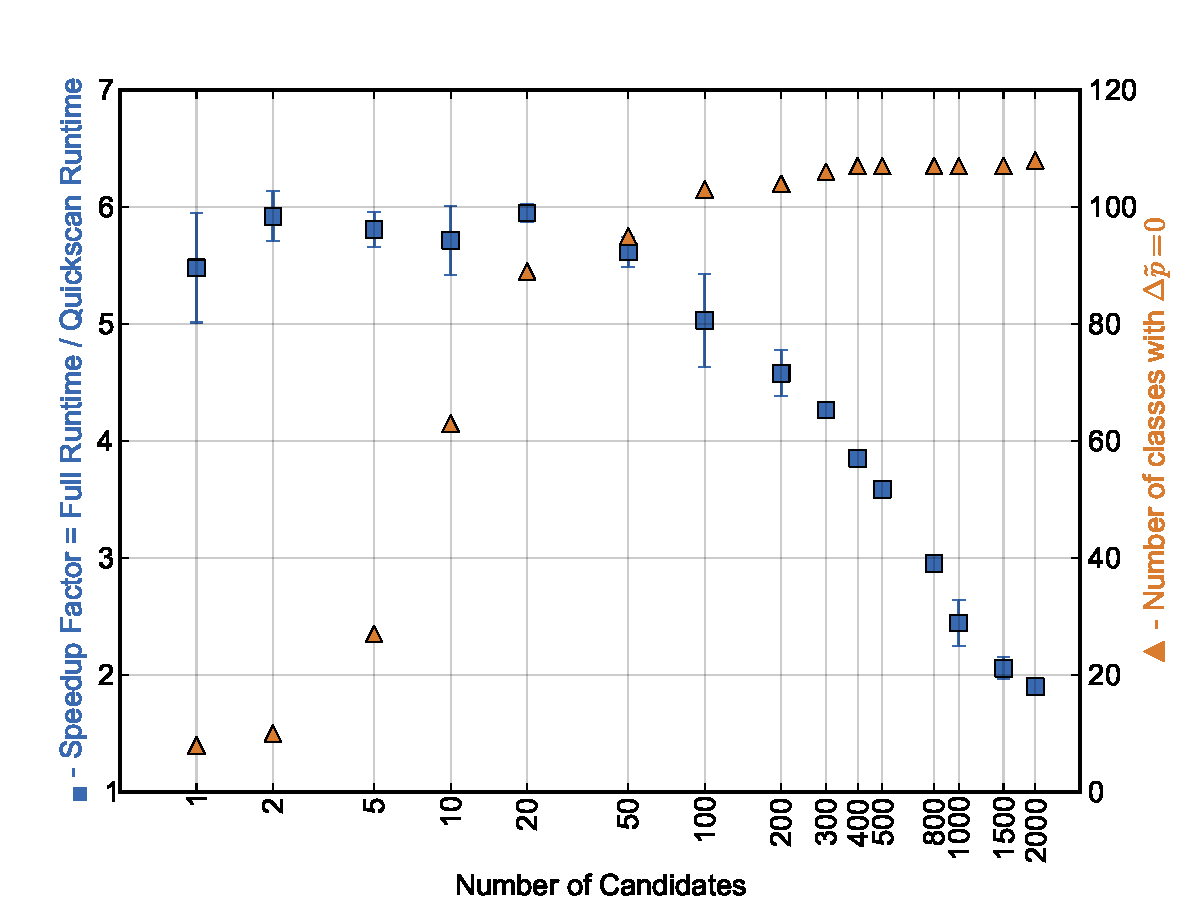
\includegraphics{parametersweep}
	\caption{Combined results of the runtime and $\Delta \ptilde$ measurement for varying numbers of Quickscan RoI candidates. The errorbars on the speedup measurement indicate the uncertainty $\sigma_{\overline T} = \sigma_T / \sqrt{N}$ on the mean $\overline T$ during the 5 trial runs. As expected with a deterministic run, there is no uncertainty of $\Delta \ptilde$.}
	\label{fig:parametersweep}
\end{figure}

\section{Analysis}
The results match the expectations: a larger number of candidates raises the chances of including the "true" RoI inside the number of candidates. This improves the accuracy of $\Delta \ptilde$, such that more classes show no deviation ($\Delta \ptilde = 0$). Thus, this observable converges to the total number of classes (108). In the same limit, the speedup value tends towards 1, which indicates that the Quickscan takes the same amount of time as the full scan in that case.

To obtain a recommendation value for \paramregions, the $\Delta \ptilde$ result should be compared with figure \ref{fig:delta_p_tilde_random_deviation}, which showed that the spread induced by random dicing only preserves $\ptilde$ for 16 classes. Taking 5 candidates, the spread induced by the Quickscan has a similar magnitude, but is only one-sided.
The illustration in figure \ref{fig:delta_p_tilde_examples} shows that for $\paramregions > 10$, the width of the distribution is negligible. 

\begin{figure}[htbp]
	\centering
	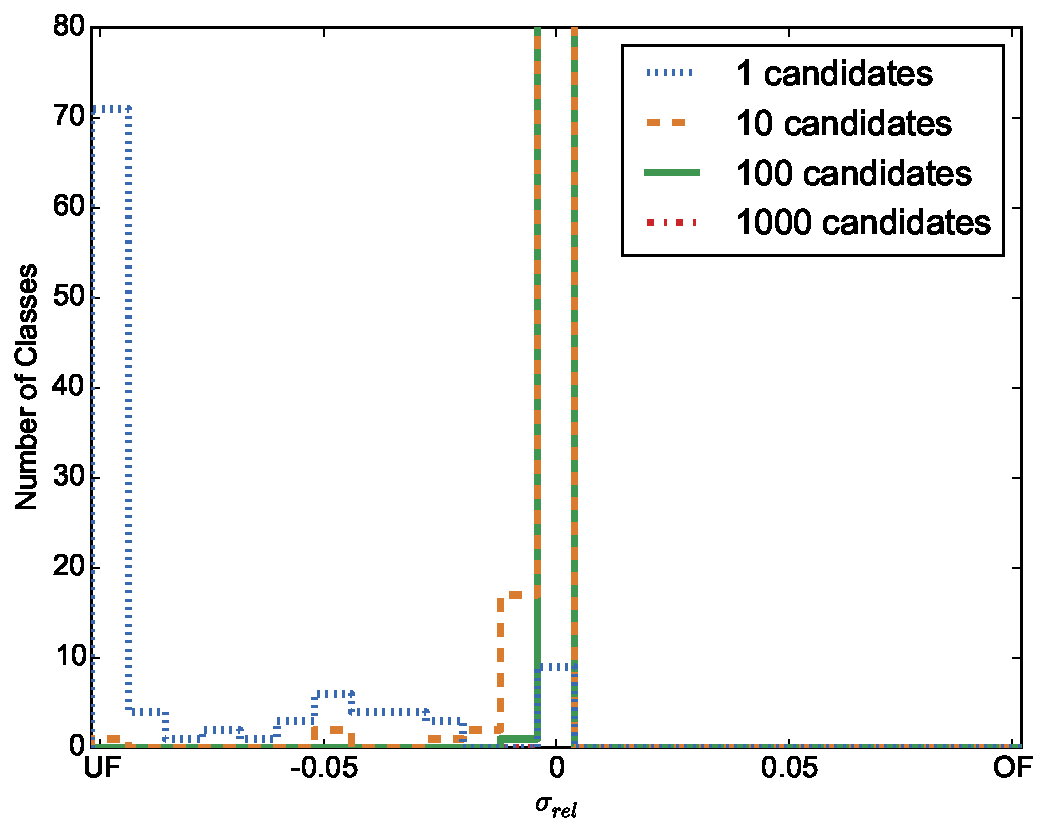
\includegraphics{delta_p_tilde_examples}
	\caption{Deviation of $\sigma_\mathrm{rel}$ due to the Quickscan algorithm. When taking more than 10 candidates, the spread is less than \unit{1}{\%} and can be neglected compared to the other random influences.}
	\label{fig:delta_p_tilde_examples}
\end{figure}


\todo{Klären, ob "fullscan" und "true" die besten Begriffe sind.}


\section{Optimization Conclusion}
Concluding, this analysis can make two suggestions for the choice of \paramregions: one could either argument conservatively and demand that the Quickscan influence becomes completely negligible. A possible choice then would be e.g. $\paramregions = 1000$, but this only provides a moderate speed-up of about 2.5 times. 
If more performance is required, one could demand that both the random influence as well as the influence induced by the Quickscan algorithm become comparable. This is the case at about $\paramregions = 10$, where the speedup is already in the saturation region of 6 times.

A sensible choice will lay somewhere in between those two extrema:
\begin{equation}
	\paramregions = 100
\end{equation}

This choice will be evaluated during the validation run in the following chapter.

% !TeX spellcheck = en_US
% !TeX encoding = UTF-8
% !TeX root = ../document.tex

\chapter{Running on a Validation Sample}
After the entire optimization has been performed on the \sumpT distribution of exclusive event classes, the validations must run on a separate subset of data. There are two options: the analysis of inclusive event classes or scanning of a different distribution. The latter option is favored and chosen because it keeps the number of event classes approximately the same. Thus, the validation run is performed on the \Minv distribution. As proposed in the previous chapter, the Quickscan number of candidate regions is fixed to $\paramregions = \num{200}$. 

The other settings for the validation run can be found in table \ref{tbl:music_configuration}. This configuration does not allow for a deterministic run, thus some random deviation of \ptilde is expected. When comparing the result of the Quickscan run with a full scan, the random deviation of \ptilde will show up as a finite width of the \sigmarel distribution. This width is then compared to a \sigmarel distribution obtained by comparing the results of two full scans.

\begin{figure}
	\centering
	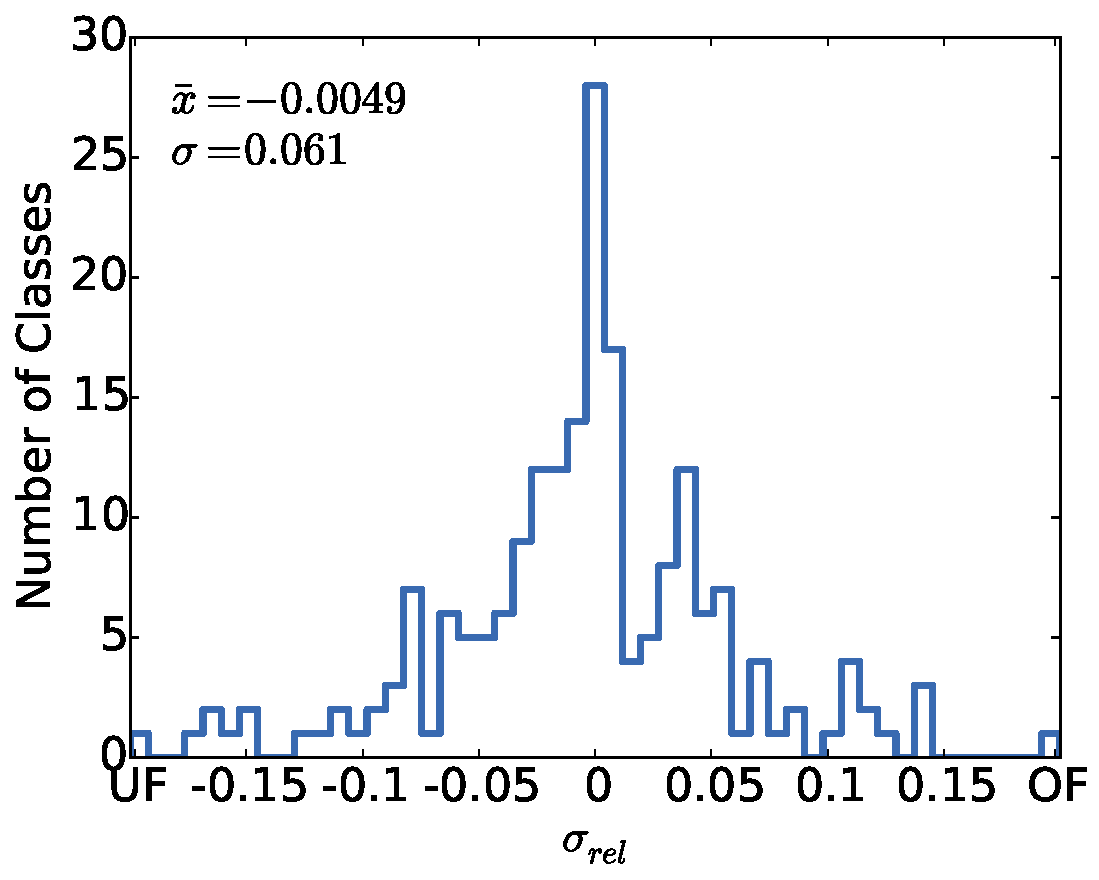
\includegraphics[width=0.49\linewidth]{delta_p_tilde_validation_random_deviation} \\
	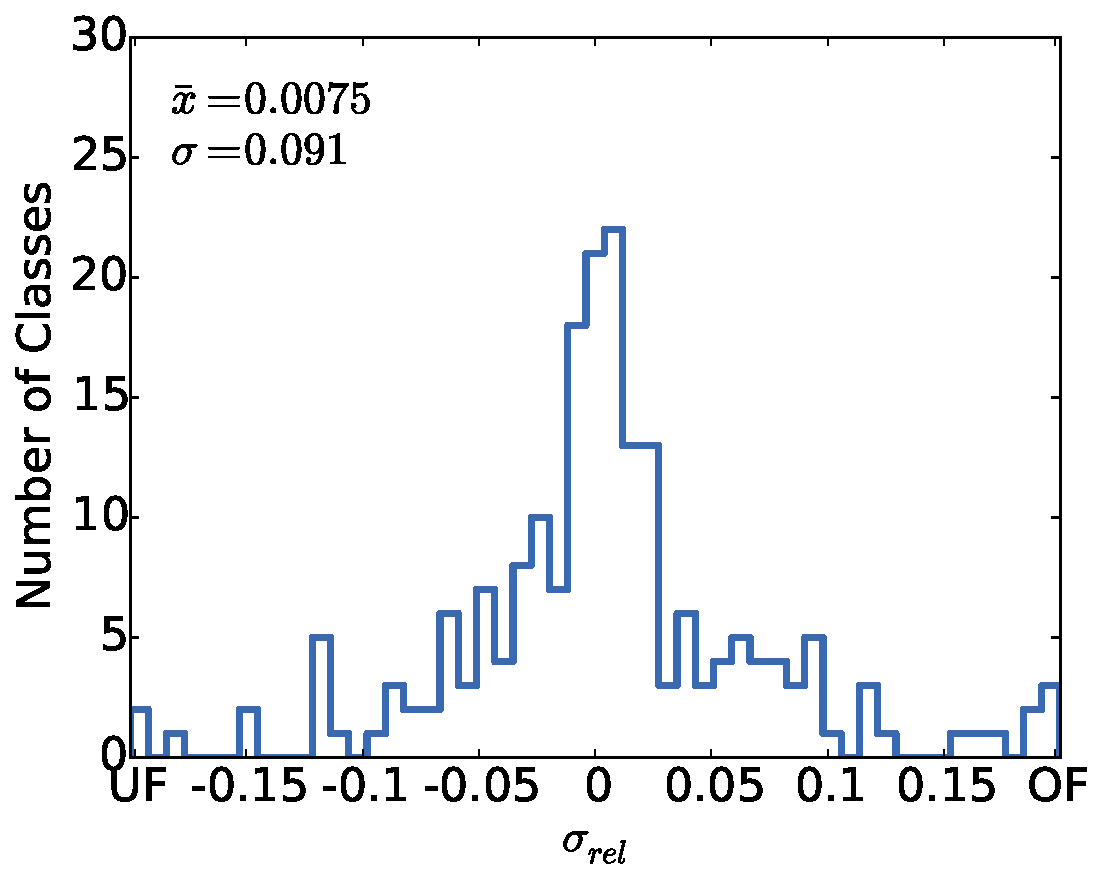
\includegraphics[width=0.49\textwidth]{delta_p_tilde_validation_f1vqs1}		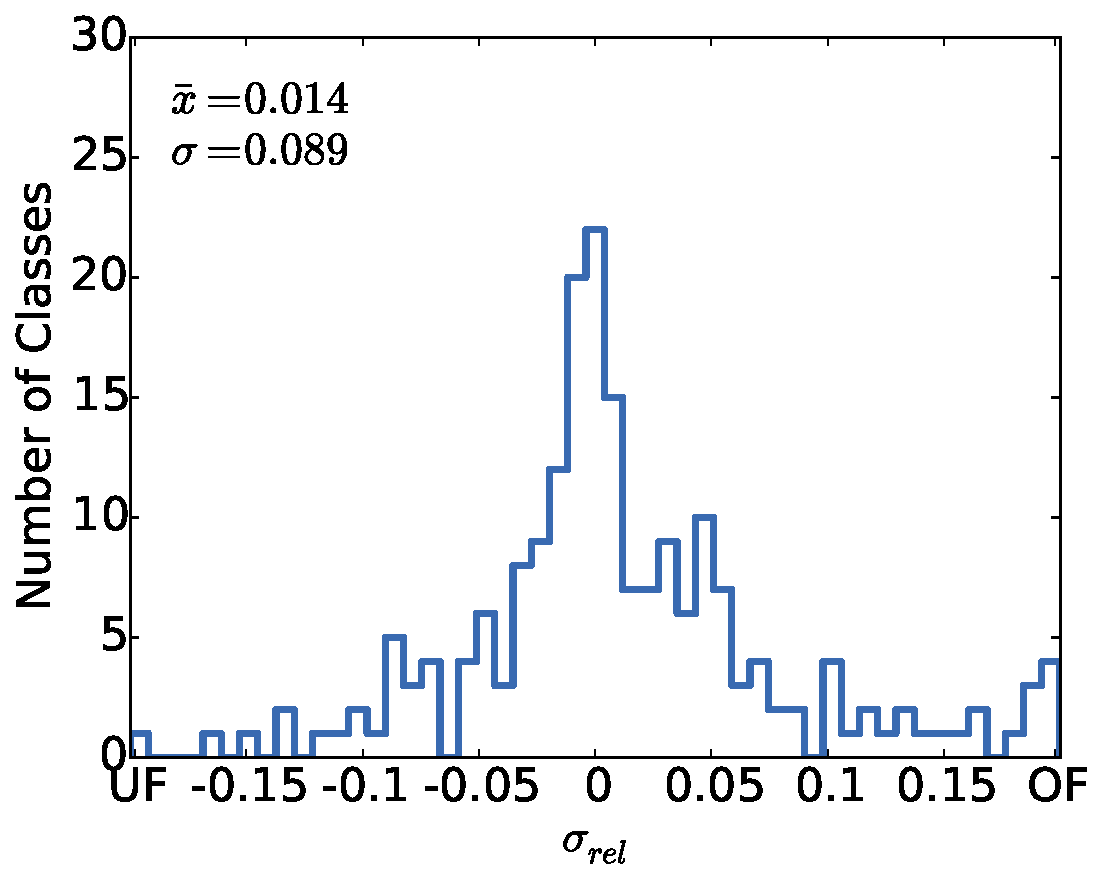
\includegraphics[width=0.49\textwidth]{delta_p_tilde_validation_f2vqs1} \\
	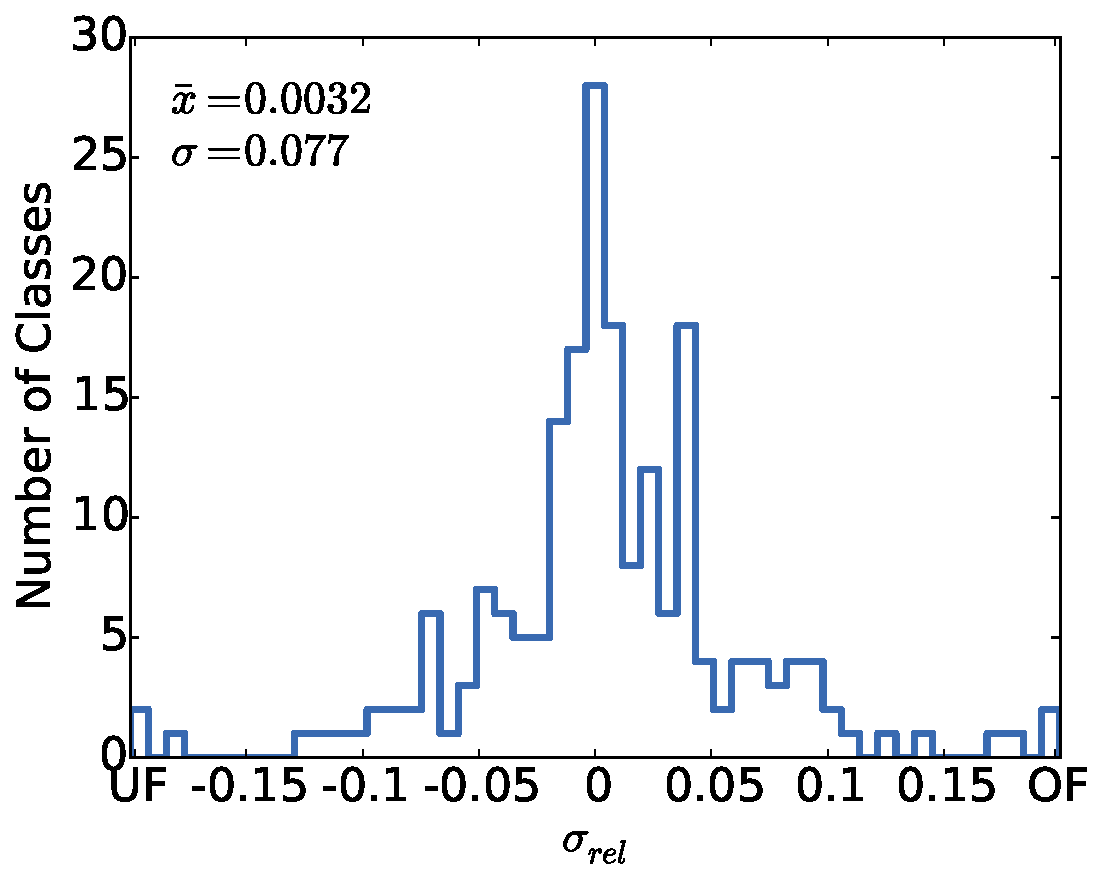
\includegraphics[width=0.49\textwidth]{delta_p_tilde_validation_f1vqs2}
	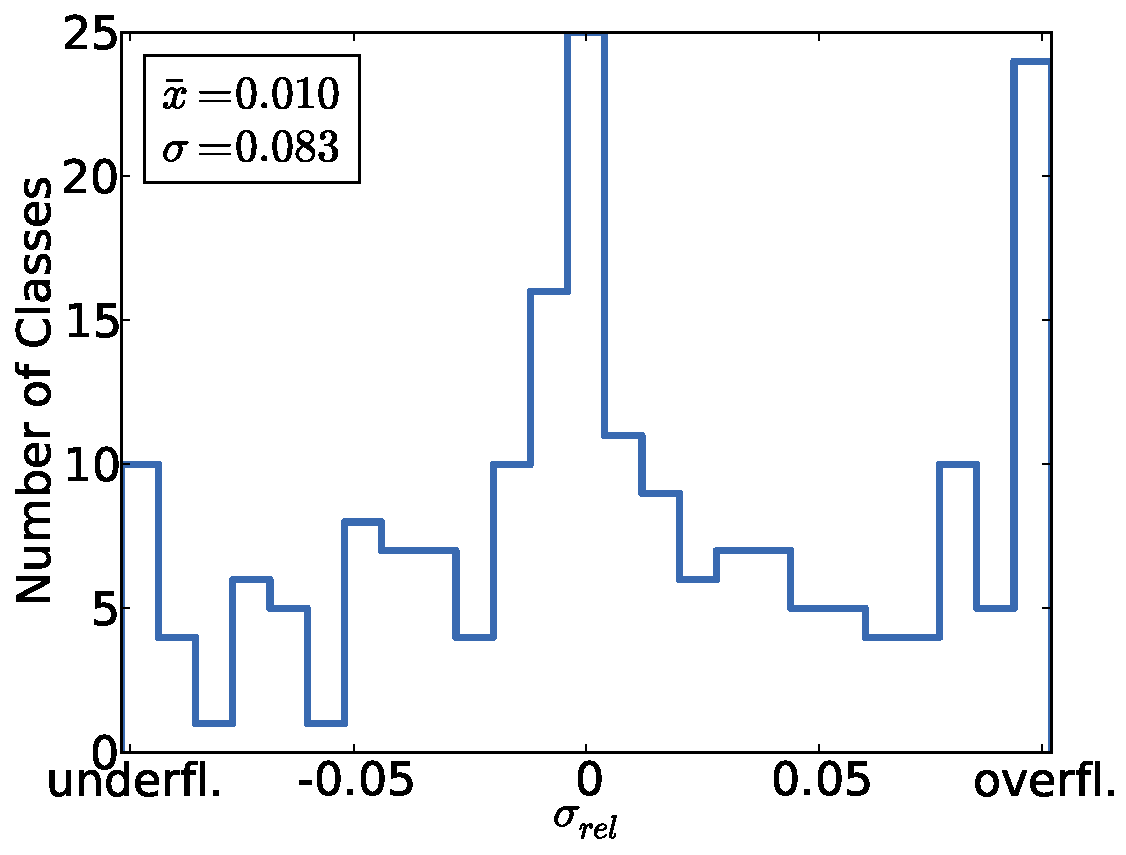
\includegraphics[width=0.49\textwidth]{delta_p_tilde_validation_f2vqs2} \\
	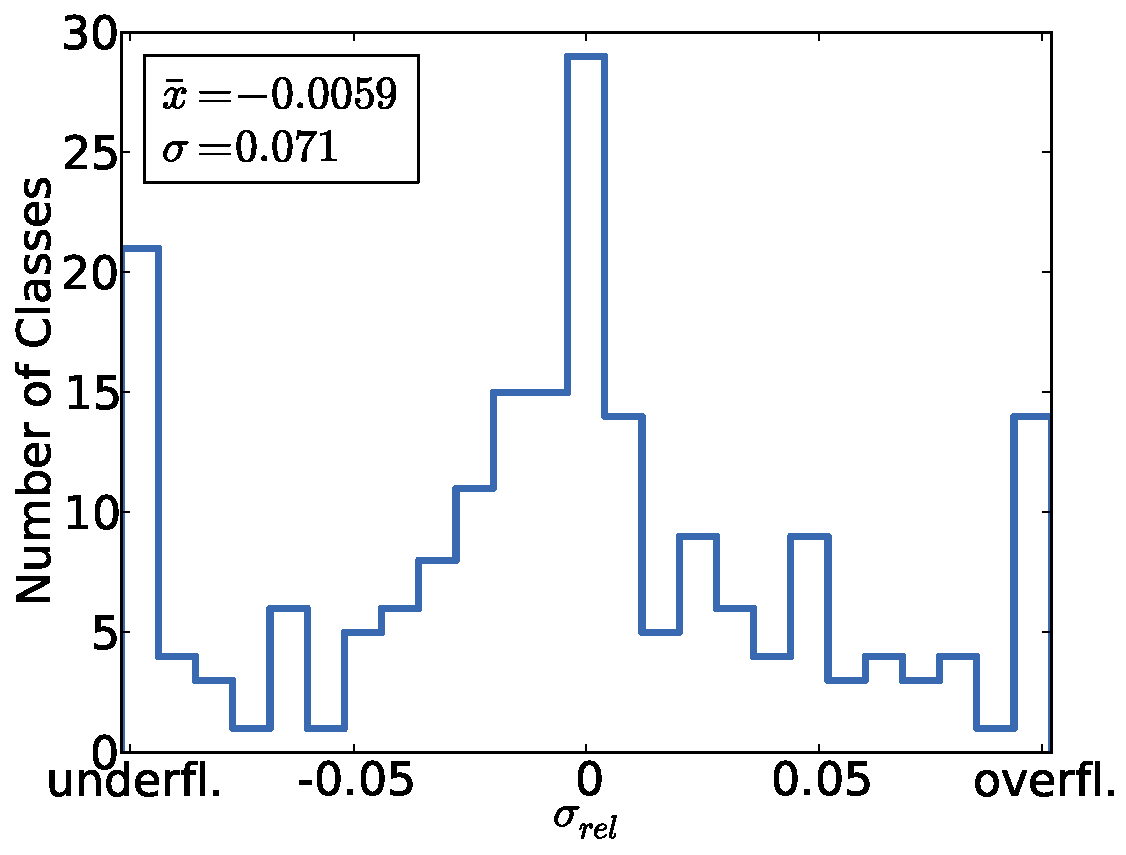
\includegraphics[width=0.49\textwidth]{delta_p_tilde_validation_f1vqs3}
	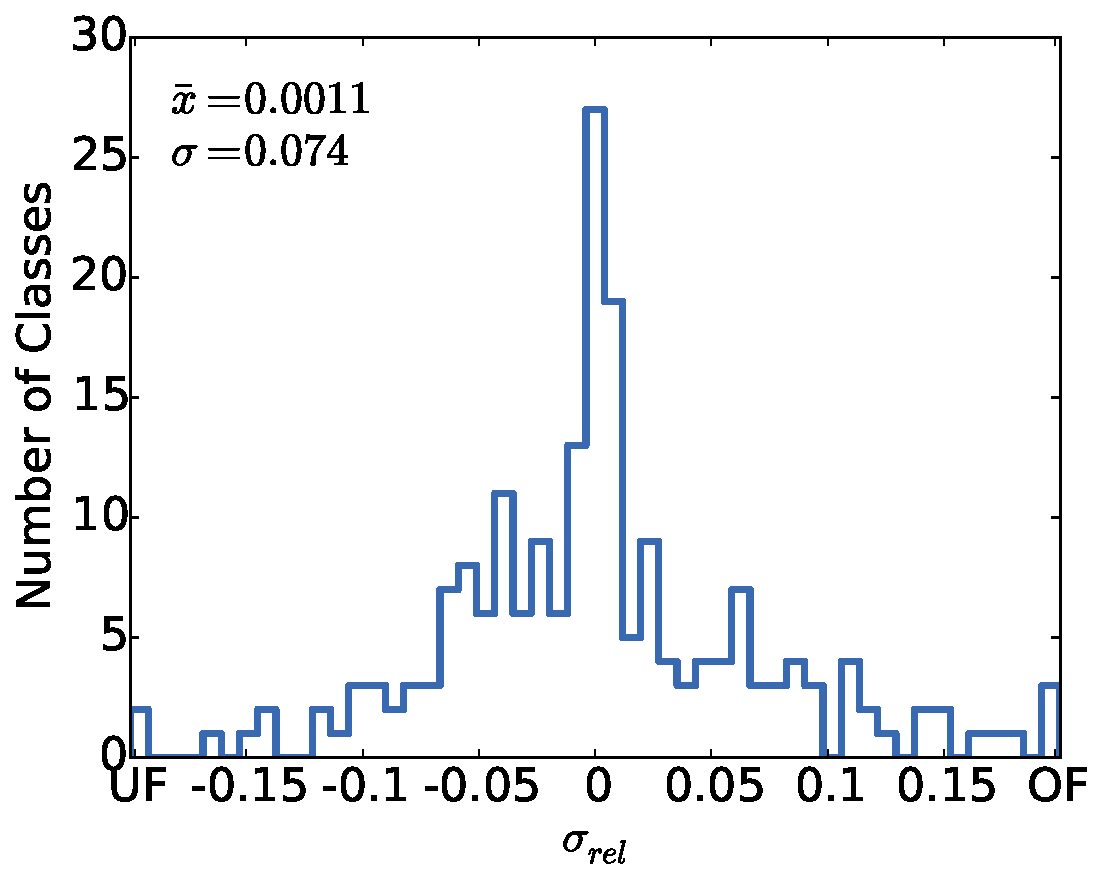
\includegraphics[width=0.49\textwidth]{delta_p_tilde_validation_f2vqs3} \\
	\caption{Distribution of the relative \ptilde deviation \sigmarel. \\Top: comparison between two full scan runs. \\Left side: comparison between full scan run \num{1} and the Quickscan runs \numrange{1}{3}. \\Right side: comparison between full scan run \num{2} and the Quickscan runs \numrange{1}{3}.}
	\label{fig:validation_result}
\end{figure}

The results of this validation run are illustrated in figure \ref{fig:validation_result}. The top figure shows the comparison between the two full scan runs. As expected, the  \sigmarel distribution shows a finite width due to random influences. The other six histograms show the comparison between the full scans and each of the three Quickscan results.
None of the distribution means is significantly shifted away from \num{0}. The distribution widths are within their deviations compatible with the broadening due to random fluctuations.

Since the number of pseudo-experiments is significantly greater in this scenario, the constant computation overhead has less influence on the computation time. As shown in table \ref{tbl:validation_speedup}, a speedup of \num{9.2 +- 0.5} times is achieved.

\begin{table}
	\centering
	\begin{tabular}{ l S l l }
		\toprule
		\multicolumn{1}{c}{} & {Measurement / \si{\second}} & {Combined / \si{\second}} & {Speedup} \\ 
		\midrule
		Full Scan 1 & 28684 & \multirow{2}{*}{\tablenum[table-format=5(4)]{30373 +- 1689}} & \multirow{5}{*}{\num{9.2 +- 0.5}} \\
		Full Scan 2 & 32062 & & \\
		\cmidrule{1-2}
		Quickscan 1 & 3386 & \multirow{3}{*}{\tablenum[table-format=5(4)]{3310 +- 52}} & \\
		Quickscan 2 & 3212 & & \\
		Quickscan 3 & 3334 & & \\
		\bottomrule
	\end{tabular}
	\caption{Results for the computation time measurement in seconds. Two full scan trials and three Quickscan trials are performed. The second column shows the combined result as mean and its error.}
	\label{tbl:validation_speedup}
\end{table}

Overall, the validation run has shown that the parameter choice $ \paramregions = \num{200} $ is reasonable. With the aid of the Quickscan, the computation time could be decreased by a factor of about \num{9} without changing the results.
% !TeX spellcheck = en_US
% !TeX encoding = UTF-8
% !TeX root = ../document.tex

\chapter{Conclusion}
The aim of this work was to develop a fast search algorithm for the MUSiC framework. After assessing the current performance situation, the concept of a region preselection step was considered. Multiple aspects of the algorithm were adapted to problems arising in the current implementation. The emerging solution is called \emph{Quickscan}. The Quickscan algorithm uses a less computation intensive estimator to assemble a list of candidate regions. Problems due to low statistics in the high-energy-tail of the kinematic distributions are suppressed by dedicated handling of nested regions. The original \p~value is subsequently only computed for the few collected candidates. The algorithm has been implemented and tested in this work. A value for the number of candidate regions, $\paramregions = \num{200}$ has been proposed here. It has been obtained by an optimization run over a wide parameter range. The choice was additionally validated over a separate subset of data. During this validation run, a performance gain of \SI{920}{\percent} was observed. This is mostly due to the smaller number of integrals which remain to be computed after the Quickscan selection.

Additionally, the Quickscan has not only been developed and validated, but also implemented and integrated into the existing MUSiC framework.

\enlargethispage{0.5cm}
\vspace{-0.2cm}
\section{Outlook}
Even though the result of this work increases scanning efficiency by almost \num{10} times, there is room for improvement:

The Quickscan algorithm could greatly benefit from an estimator that improves handling of regions with $\Nmc < \num{3}$. A possible solution could be to use a Poisson distribution around the number of MC events and calculate its \p~value back to a Gaussian statistic before combining with the systematical uncertainty. This could lead to a better mathematical understanding of the algorithm, especially since the ad-hoc nested region handling may turn out to be superfluous.

Furthermore, the parallelization of the general scanning algorithm could be improved. The correlated dicing of the pseudo-experiments requires communication between the worker tasks. The correlation could instead be handled by a fixed seed of the worker's pseudo-random number generators. This would make the scanning step trivially parallelizable (either over the classes or over the pseudo-experiments), enabling it to run on a computing grid instead of the 64-core MUSiC host.



\cleardoublepage
\bibliographystyle{utphys}
\bibliography{bibliography,images}

\cleardoublepage
% !TeX spellcheck = en_US
% !TeX encoding = UTF-8
% !TeX root = ../document.tex


\renewcommand\thechapter{A}
\chapter{Appendix}

\section*{Time per Integral}
\begin{table}
	\centering
	\begin{tabular}{ S S S S }
		\toprule
		{Histograms} & {Number of integrals} & {Total runtime / \si{\second}} & {per integral / \si{\micro\second}} \\
		\midrule
		% /home/home1/institut_3a/lieb/MUSiC-work/Scan/2015-05-05/12_CompleteOutput/output.txt
		%2369 & 23110209 & 5179.87 & 224 \\
		% /home/home1/institut_3a/lieb/MUSiC-work/Scan/2015-05-05/02_FullRef/report.txt
		%18991 & 81734778 & 16983.60 & 207 \\
		
		2369 & 23110209 & 5179.87 & 224.1 \\      
		2374 & 23146885 & 5190.3 & 224.2 \\       
		2390 & 22968240 & 5198.89 & 226.4 \\      
		2375 & 23089566 & 5218.37 & 226.0 \\      
		2355 & 22741383 & 5204.23 & 228.8 \\      
		2357 & 23079630 & 5172.68 & 224.1 \\      
		2377 & 23119389 & 5183.55 & 224.2 \\      
		2389 & 23208732 & 5194.77 & 223.8 \\      
		2361 & 23288752 & 5221.18 & 224.2 \\      
		2368 & 22925427 & 5217.4 & 227.6 \\
		18991 & 81734778 & 16983.6 & 207.8 \\     
		19017 & 80847194 & 16970.2 & 209.9 \\     
		18945 & 80976157 & 16990.5 & 209.8 \\     
		18993 & 81748828 & 16987.3 & 207.8 \\     
		19079 & 81471964 & 16985.9 & 208.5 \\     
		18853 & 81188030 & 16982 & 209.2 \\       
		18906 & 81149116 & 17019.2 & 209.7 \\     
		18960 & 81354379 & 17003.4 & 209.0 \\     
		18976 & 81185262 & 16967.9 & 209.0 \\     
		19089 & 81772747 & 16987.6 & 207.7 \\
		\bottomrule
	\end{tabular}
	\caption{Benchmarking results of the original scanning process. The timing has been measured on a data subset, using a single CPU and includes setting up the process and writing out the results. The agreement of the time per integral between the runs motivates the rough estimate of \SI{200}{\micro\second} per integral.}
	\label{tbl:motivation_timing}
\end{table}

\newpage
\section*{MUSiC Scanner Configuration}
\begin{table}
	\centering
	\begin{tabular}{ l l l }
		\toprule
		& optimization & validation \\ 
		\midrule
		data & \multicolumn{2}{c|}{2012, $\sqrt{s} = \SI{8}{\TeV}$} \\ 
		luminosity & \multicolumn{2}{c|}{ $L = \SI{19.7}{\per\femto\barn}$ } \\ 
		\midrule
		event classes & excl. & excl. \\ 
		distribution & \sumpT & \Minv \\
		N-jet threshold & \num{2} & - \\
		\p~threshold & \num{0.3} & \num{0.3} \\
		dicing rounds & \num{1000} & \num{100000} \\
		hits threshold & - & \num{100} \\
		Fill-Up & yes & yes \\
		\bottomrule
	\end{tabular}
	\caption{MUSiC configuration values for the optimization and validation runs.}
	\label{tbl:music_configuration}
\end{table}

\newpage
\section*{Optimization \ptilde Results}
\begin{table}
	\centering
	\begin{tabular}{ 
			S[table-format=4]
			S[table-format=3]
			S[table-format=3.1]
		}
		\toprule
		\paramregions & \multicolumn{1}{c}{Classes with $\Delta \ptilde = 0$} & \multicolumn{1}{c}{Percentage of total classes} \\
		\midrule
		1 & 8 & 7.4 \\ 
		2 & 10 & 9.3 \\ 
		5 & 27 & 25.0 \\ 
		10 & 63 & 58.3 \\ 
		20 & 89 & 82.4 \\ 
		50 & 95 & 88.0 \\ 
		100 & 103 & 95.4 \\ 
		200 & 104 & 96.3 \\ 
		300 & 106 & 98.1 \\ 
		400 & 107 & 99.1 \\ 
		500 & 107 & 99.1 \\ 
		800 & 107 & 99.1 \\ 
		1000 & 107 & 99.1 \\ 
		1500 & 107 & 99.1 \\ 
		2000 & 108 & 100.0 \\ 
		\bottomrule
	\end{tabular}
	\caption{Result of the optimization $\Delta \ptilde$ measurement. There are 108 classes in total for which the $\ptilde$ value is computed and as such for which the Quickscan is applied. All 5 trial runs yield exactly the same results, thus they are not separately listed here.}
	\label{tbl:deltaptilde_results}
\end{table}

\newpage
\section*{Optimization Timing Results}
\begin{table}
	\centering
	\begin{tabular}{ 
			S[table-format=4] 
			S[table-format=4] 
			S[table-format=4] 
			S[table-format=4] 
			S[table-format=4]  
			S[table-format=4] 
			S[table-format=4(2)] 
			S[table-format=1.1(1)]
		}
		\toprule
		\paramregions & {$T_1$ / \si{\second}} &  {$T_2$ / \si{\second}} & {$T_3$ / \si{\second}} & {$T_4$ / \si{\second}} & {$T_5$ / \si{\second}} & {$\overline{T} \pm \Delta T$} & {Speedup} \\
		\midrule
		{Full} & 5379 & 5500 & 5331 & 5371 & 5396 & 5395 +- 28 & 1.0 +- 0.0 \\ 
		\midrule
		1 & 1460 & 880 & 973 & 912 & 885 & 1022 +- 111 & 5.3 +- 0.6 \\ 
		2 & 1054 & 870 & 871 & 900 & 886 & 916 +- 35 & 5.9 +- 0.2 \\ 
		5 & 945 & 1038 & 898 & 909 & 869 & 932 +- 29 & 5.8 +- 0.2 \\ 
		10 & 1142 & 861 & 985 & 907 & 879 & 955 +- 51 & 5.7 +- 0.3 \\ 
		20 & 930 & 886 & 889 & 919 & 913 & 907 +- 9 & 5.9 +- 0.1 \\ 
		50 & 940 & 1073 & 952 & 937 & 915 & 963 +- 28 & 5.6 +- 0.2 \\ 
		100 & 1555 & 987 & 1031 & 993 & 975 & 1108 +- 112 & 4.9 +- 0.5 \\ 
		200 & 1406 & 1120 & 1111 & 1171 & 1130 & 1188 +- 56 & 4.5 +- 0.2 \\ 
		300 & 1251 & 1330 & 1251 & 1248 & 1247 & 1265 +- 16 & 4.3 +- 0.1 \\ 
		400 & 1373 & 1507 & 1375 & 1395 & 1364 & 1403 +- 27 & 3.8 +- 0.1 \\ 
		500 & 1474 & 1594 & 1489 & 1481 & 1487 & 1505 +- 22 & 3.6 +- 0.1 \\ 
		800 & 1792 & 1860 & 1826 & 1816 & 1846 & 1828 +- 12 & 3.0 +- 0.0 \\ 
		1000 & 3254 & 2045 & 2064 & 2022 & 2041 & 2285 +- 242 & 2.4 +- 0.3 \\ 
		1500 & 3203 & 2544 & 2505 & 2466 & 2518 & 2647 +- 140 & 2.0 +- 0.1 \\ 
		2000 & 2971 & 2765 & 2820 & 2787 & 2863 & 2841 +- 36 & 1.9 +- 0.0 \\ 
		\bottomrule
	\end{tabular}
	\caption{Result of the optimization computation time measurement. The numbers show the wall-clock time. The combined result $\overline{T} \pm \Delta T$ consist of the sample mean ${\overline{T} = \frac{1}{N} \sum_i T_i}$ and its deviation ${\Delta T = \frac{1}{\sqrt{N}} \sqrt{\frac{1}{N} \sum_i (T_i - \overline{T})^2}}$. As expected, the wall-clock time is subject to fluctuations of about \SIrange{1}{10}{\percent}. The resulting speedup $\frac{T_{\textrm{Full}}}{T_{\textrm{QS}}}$ is calculated using the mean values and is up to 5.9 times.}
	\label{tbl:timing_results}
\end{table}


\cleardoublepage
% !TeX spellcheck = de_DE
% !TeX encoding = UTF-8
% !TeX root = ../document.tex

\chapter*{Danksagung}
Ich möchte mich ganz herzlich bei allen Menschen bedanken, die mir beim Erstellen dieser Arbeit zur Seite standen. 

Das behandelte Thema schlägt eine Brücke zwischen meinem Studium, der Teilchenphysik, und meinem Hobby, der Software. Für diese Möglichkeit und die Unterstützung während des Verfassens der Arbeit danke ich ganz besonders Herrn Professor Thomas Hebbeker.

Am III. Physikalischen Institut wurde ich als Bachelor sehr herzlich aufgenommen und danke dafür allen Mitgliedern der Aachen-IIIA-CMS-Gruppe. Besonders lebhafte Erinnerungen werde ich dabei an das MUSiC-Büro, bestehend aus Deborah Duchardt, Simon Knutzen, Tobias Pook und Andreas Albert, haben. Durch das Beantworten hunderter Fragen hat die gesamte Physikergruppe mein Physik- und Wissenschaftsverständnis "signifikant" "geboostet".

Explizit möchte ich Simon Knutzen und Deborah Duchardt dafür danken, dass sie mich bei der Entwicklung des Quickscans in die richtige Richtung geleitet haben und meine Arbeit im Anschluss probegelesen haben.

Des Weiteren möchte ich mich für das finale Korrekturlesen der Arbeit und für hilfreiche Hinweise und Unterstützung während der Präsentationen bei Dr. Arnd Meyer bedanken. Ebenfalls danke ich Herrn Professor Martin Erdmann, der sich bereit erklärt hat, diese Arbeit als Zweitkorrektor zu betreuen und mich zuvor mit den Vorlesungen der Teilchenphysik für eine Bachelorarbeit in diesem Feld begeistern konnte.

Abschließend bedanke ich mich bei meiner Familie, meiner Freundin, meinen Freunden und meinen Mitbewohnern für die mentale Unterstützung, die ich in sowohl in den stressigeren letzten Monaten, als auch im Rest des Studiums genießen konnte.

%Thomas Hebbeker
%Martin Erdmann
%Arnd Meyer
%MUSiC Group:
%	Simon Knutzen
%	Deborah Duchardt
%	Tobias Pook
%	Andreas Albert
%CMS Group in Aachen
%Friends \& Family

\end{document}